\documentclass[a4paper,11pt]{article}
\usepackage[T1]{fontenc}
\usepackage[utf8]{inputenc}
\usepackage{lmodern}
\usepackage[francais]{babel}
\usepackage[ portrait, margin = 0.7 in]{geometry}

\usepackage{amsmath}
\usepackage{amssymb}

\usepackage{mathrsfs}  
\usepackage{dutchcal}
\usepackage{graphicx}

\graphicspath{{./images/}}
\usepackage{float}
\usepackage{subfig}
\usepackage{wrapfig}

\usepackage{gensymb}
\usepackage{multicol, caption}
\usepackage{makecell}
\usepackage{bm}
\numberwithin{equation}{section}

\usepackage{hyperref}
\usepackage{breakcites}

%In order to have figures on just one column
\newenvironment{Figure}
  {\par\medskip\noindent\minipage{\linewidth}}
  {\endminipage\par\medskip}

\DeclareMathOperator{\arccosh}{arccosh}

\begin{document}

\makeatletter
\begin{titlepage}
    \begin{center}
        \vspace*{1cm}
      
          {\Large \textbf{Amélioration et validation du code de caractérisation d'amas de galaxies PROF-CL pour la mission EUCLID}}
        
        \vspace{0.5cm}
        {\large Pour le diplôme de Master 1 Astronomie et Astrophysique, "Sciences de l’Univers et Technologies Spatiales". Observatoire de Paris}
        
        \vspace{1.5cm}
        
        \textbf{Mercier Wilfried}
        

        Sous la direction de Mamon Gary
        
        \vspace{0.5cm}
        \@date
        
        \vfill
      
        
      %  \includegraphics[width=0.4\textwidth]{university}
        
        Institut d'Astrophysique de Paris\\
        Observatoire de Paris\\
        
    \end{center}
\end{titlepage}
\makeatother

\newpage

\begin{center}
  \section*{Résumé}
\end{center}

    Une nouvelle version du code de caractérisation d'amas de galaxies PROFCL est codée prenant en compte les amas académiques et ceux d'AMICO. Le code fonctionne en mode circulaire et/ou elliptique avec et sans fond. De nouvelles équations sont calculées pour la probabilité de position des galaxies dans le cas elliptique. Le code principal a été modifié pour pouvoir améliorer la convergence des algorithmes de minimisation non-contraints en ajoutant dans le \textit{likelihood} deux fonctions pénalité différentes; une étant plus générale que l'autre. Une méthode de détermination du rayon caractéristique par séparation médiane est implémentée et comparée aux méthodes par maximum de vraisemblance. Le code est testé sur les mocks académiques et sur $\sim 550$ amas AMICO. On trouve des performances correctes en terme de biais pour $N \gtrsim 50$ galaxies à la fois en elliptique et en circulaire pour le \textit{log scale radius}, l'ellipticité et le $PA$. La richesse est légèrement biaisée négativement vers $-0.2 \rm{dex}$ ce qui est probablement dû à une surévaluation du fond. Globalement $DE$ trouve de meilleurs résultats que $TNC$ bien que la différence soit moins notable sur les amas AMICO. Des améliorations futures du code tel que le \textit{deblending} sont discutées en conclusion.


\newpage

\tableofcontents

\newpage

\section*{Notations}
\addcontentsline{toc}{section}{Notations utiles}
\begin{tabular}{l l l}
  Nom & Symbole(s) & Description \\
  Profil NFW & $\rho_{NFW}$ & Profil de densité universel de matière noire Navarro, Frenk, White \\
  Densité surfacique & $\Sigma (R)$ & Densité surfacique projetée sur le ciel \\
  Rayon de pente -2 &  $r_s$ , $r_{-2}$ & Rayon pour lequel la pente de $\rho_{NFW}$ vaut -2 \\
  & $r_{200}$ & Rayon pour lequel la densité de la sphère vaut 200 fois la densité \\
  & & moyenne de matière dans l'Univers \\
  Rayon viriel & $r_{vir}$ & Rayon pour lequel la matière dans la sphère est en équilibre \\
  Rayon projeté & $R$ & Distance au centre d'un amas projetée sur le ciel \\
  Rayon circularisé & $\mathscr{R}$ & Distance projetée au centre d'un amas après circularisation \\
  Ellipticité & $e$ & Ellipticité de l'amas égale à $1 - b/a$ avec b le demi-petit axe et \\
  & & a le demi-grand axe \\
  Angle de position & $PA$ & Angle entre le demi-grand axe et le Nord allant du Nord vers l'Est \\
  & $\bm{\theta}$ & Vecteur des paramètres du modèle \\
  Nombre projeté & $N_p (R)$ & Nombre de galaxies à une distance projetée $R$ du centre de l'amas \\
  Richesse & $N_{\rm{eff}}$ & Somme des probabilités d'appartenance des galaxies à l'amas \\
  
\end{tabular}

\section*{Avant propos}
\addcontentsline{toc}{section}{Avant propos}
Dans la suite les termes halos et amas seront utilisés pour décrire la même chose, à savoir des amas de galaxies. Pour éviter toute confusion le terme halo sera exclusivement utilisé pour désigner les amas de galaxies issus de la simulation \cite{Catalog_EUCLID}.\par
A l'inverse le terme amas référera uniquement soit aux amas "académiques" (mocks académiques) simulés lors du stage pour tester l'efficacité du code, soit aux amas trouvés par l'algorithme de détection d'amas AMICO. \par
Les expressions latines et la terminologie en anglais seront écrites en italique dans ce qui suit.\newline \par

L'ensemble du travail et du traitement de données a été effectué en python avec les bibliothèques \textit{numpy}\footnote{\url{https://docs.scipy.org/doc/}} et \textit{astropy}\footnote{\url{http://docs.astropy.org/en/stable/}}


\newpage

\section{EUCLID, AMICO et PROFCL}
  \subsection{Projet EUCLID}
    PROFCL a pour but de fonctionner à terme sur des données issues du future satellite EUCLID de l'Agence Spatial Européenne (ESA). Cette mission cherche à mieux comprendre la nature de l'énergie sombre et l'origine de l'expansion accélérée de l'Univers en étudiant notamment les lentilles gravitationnelles faibles ainsi que la distribution spatiale des amas de galaxies et leurs propriétés.\newline
    Pour ce faire, un large catalogue de $15000 \ \ \rm{deg^2}$ (\textit{wide survey}) d'objets extra-galactiques à la fois dans les bandes optiques jusqu'à $24.5 \rm{mag}$ et dans l'infrarouge proche (bandes Y, J, H) jusqu'à $24 \rm{mag}$ sera disponible, complémenté par deux catalogues plus restreints (\textit{deep surveys}) cumulant $40\rm{deg^2}$ et pouvant aller jusqu'à $26 \rm{mag}$ environs\cite{EUCLID}. Tous les objets observés posséderont un redshift photométrique, voir un redshift spectroscopique pour certains d'entre eux. EUCLID sera en mesure d'observer des galaxies de masse supérieure à $10^{14} \rm{M_{\odot}}$ et jusqu'à des redshifts de l'ordre de $2$.\par
    L'étude conjointe des lentilles gravitationnelles faibles (\textit{Weak Lensing} - WL) et des amas de galaxies (\textit{Galaxy Clustering} - GC) devrait permettre en particulier d'étudier certaines questions de cosmologie contemporaine, parmi lesquelles se trouvent\cite{EUCLID_BIBLE}:
    \begin{itemize}
      \item la dépendance en redshift du paramètre $w(a)$ où $a = 1 + z$ et de sa dérivée première $w_a (a) = dw/da$ de l'équation d'état de l'énergie sombre $p = w(a) \rho$
      \item le facteur de croissance et sa dérivée (\textit{growth rate}) $f(z) = [ \Omega_m (z) ]^{\gamma}$ qui caractérisent l'efficacité à former des structure dans l'Univers au cours du temps, en particulier la mesure de l'exposant $\gamma$
    \end{itemize}
  
  \subsection{Algorithmes de détection d'amas: AMICO et PZWav}
    Afin de pouvoir étudier le GC et en déduire des informations sur la cosmologie, la première étape consiste à détecter les amas de galaxies dans le catalogue d'EUCLID. Dans ce contexte, des algorithmes de détection d'amas (\textit{cluster finders}) ont été développés et testés dans un ensemble de 4 challenges (CFC).\newline
    Chaque algorithme a été testé sur un catalogue mock\cite{Catalog_EUCLID} d'une taille originelle de $500 \rm{deg^2}$ réduite à $300 \rm{deg^2}$ fournissant des données similaires à celles attendues pour EUCLID. En particulier le catalogue était limité à des objets plus brillants que $24 \rm{mag}$ dans les intervalles considérés de masse et de redshift. Les positions des galaxies étaient fournies avec un redshift photométrique et une probabilité de distribution associée. Comme pour EUCLID, un second catalogue de $20 \rm{deg^2}$ était fourni avec à la fois des redshifts spectroscopiques et photométriques.\par
    Parmi les 8 codes de départ, deux ont été retenus pour leur efficacité et leur complémentarité dans les intervalles de masse et de redshift où ils excellent : PZWav et Adaptative Matched Identifier of Clustered Objects (AMICO).\par

    Seules les données d'AMICO ont pu être utilisées et analysées pendant le stage. Ainsi, on ne donnera qu'une description très brève du fonctionnement de PZWav (voir \cite{EUCLID} et \cite{IRAC} pour plus d'informations sur le fonctionnement de l'algorithme).
    \subsubsection{PZWav}
      Cet algorithme découpe l'intervalle de redshift en plusieurs tranches puis construit à l'aide de la densité de probabilité des cartes de densités à différents redshift. En répétant l'opération avec des densités de probabilité aléatoires une valeur maximale sur le bruit du fond peut être déduite ainsi que sa variation avec le redshift. Les amas sont alors détectés comme des pics dans les cartes de densité et une valeur du rapport signal-bruit ($S/N$) est déduite.
    \subsubsection{AMICO}
      AMICO est un algorithme de détection d'amas basé sur une méthode de Filtrage Optimale (OF) originellement utilisé pour la détection d'amas sur des données de lentille gravitationnelle faible\cite{AMICO}. Les données sont décrites comme étant la somme d'un modèle et d'un fond non-uniforme. 
	  La densité surfacique du fond est calculée localement autour de chaque grande structure mais suffisamment loin pour ne pas prendre en compte le signal provenant du modèle.\newline      
      L'amplitude du signal brut (sans fond) est alors déterminée en appliquant un filtre sur la distribution des galaxies; les pics dans la carte de densité 3D obtenue correspondent aux amas. Un processus itératif va alors:
	\begin{itemize}
		\item éliminer tous les pixels de l'image avec un rapport signal-bruit $S/N$ inférieur à une certaine limite $(S/N)_{\rm{min}}$ typiquement de l'ordre de 2
		\item chercher le pic avec la plus grande amplitude et l'assigner comme étant un amas
		\item assigner une probabilité $p(i \in j)$ d'appartenance de la galaxie i à l'amas j pour toutes les galaxies au voisinage de l'amas ainsi qu'une "probabilité de champ" (\textit{field probability}) définie comme $p_{f,i} = 1 - \sum_{j=1}^N p(i \in j)$
		\item retirer de l'image le signal du modèle pour chaque galaxie multiplié par la probabilité  de champ
		\item recommencer depuis l'étape 1 jusqu'à ce que plus aucune galaxie n'ait $S/N > (S/N)_{\rm{min}}$
	\end{itemize}	      
       
      Contrairement à PZWav cet algorithme possède l'avantage de fournir une probabilité d'appartenance à l'amas (\text{membership}) que l'on pourra incorporer dans le calcul du likelihood (voir section \ref{sec:Likelihood}). En principe AMICO permet de mieux détecter les petites structures, cependant comme montré dans \cite{EUCLID} cet algorithme a aussi le défaut d'avoir un taux de fragmentation\footnote{Proportion de halos (issus de la simulation) détectés comme étant composés de plusieurs amas} plus élevé que les autres algorithmes.
      
    \subsection{PROFCL: code de détermination des propriétés d'amas par maximum de vraisemblance}

    
      PROFCL est un algorithme qui cherche à déterminer les meilleurs paramètres des amas détectés par AMICO et PZWav par maximum de vraisemblance. Le code ne reçoit en entrée que les positions des galaxies appartenant aux amas trouvés ainsi que les probabilités d'appartenance à l'amas pour AMICO. \par
      À chaque galaxie de l'amas détecté va être associée une probabilité de trouver la galaxie à cette position sachant les paramètres considérés. On peut alors définir un \textit{likelihood} comme étant le produit des probabilités de toutes les galaxies de l'amas. Le code va alors se charger de trouver les paramètres qui minimisent l'opposé du logarithme du \textit{likelihood} via plusieurs procédures de minimisation (descente de gradient, algorithme stochastique, simplex, etc...).\newline
      Les paramètres testés par PROFCL sont les suivants:
      
      \begin{itemize}
        \item Rayon caractéristique et en particulier son logarithme (\textit{log scale radius}) noté $\log_{10} (r_s/\rm{arcmin})$
        \item Angle de position de l'amas en degrés noté $PA$
        \item Ellipticité de l'amas $e = 1 - b/a$
        \item Densité surfacique du fond $\Sigma_{\rm{bg}}$ supposée constante en $\rm{arcmin^{-2}}$
        \item Le logarithme du rayon de troncation $\log_{10} ( R_{\rm{trunc}} / \rm{arcmin})$ si un modèle NFW tronqué est testé
      \end{itemize}
	
	\subsection{Fonctionnalités déjà incluses et améliorations à apporter}
		Au moment de commencer le stage, PROFCL était dans sa version 1.10. Les fonctionnalités principales avaient déjà été programmées mais le code n'avait été que peu testé jusqu'à présent. En principe, le code était capable de fonctionner dans les cas suivants:
		\begin{itemize}
			\item amas circulaire : considère $e, PA, N_{\rm{bg}} = 0$  et retourne $\log_{10}(r_{-2})$
			\item amas elliptique : retourne $\lbrace e, PA, \log_{10}(r_{-2}) \rbrace$
			\item avec fond : retourne en plus $\log_{10} (\Sigma_{\rm{bg}})$
		\end{itemize}
		
		Le cas elliptique pouvait être traité par approximation analytique de l'intégrale de densité de surface (cf. section \ref{Densité_surfacique_projetée}) ou par Monte-Carlo. Le code ne fonctionnait que sur les amas académiques d'Artis.\newline
		Dans la pratique, certaines parties du code n'étaient pas opérationnelles ou ne retournaient pas les résultats attendus. Il a donc fallu retravailler dessus avant de pouvoir analyser les performances du code. Ci-dessous une liste non-exhaustive des parties du code sur lesquelles il a fallu retravailler/implémenter:
		\begin{itemize}
			\item Ré-écriture de la séparation médiane
			\item Ré-écriture et implémentation des équations de la probabilité pour des amas elliptiques (potentiellement décentrés)
			\item Gestion des sorties de limites pour des algorithmes sans contraintes (cf. annexe \ref{Algo})
			\item Analyse des performances sur les mocks académiques
			\item Gestion et analyse des données issues d'AMICO
		\end{itemize}

\begin{figure}
    \vspace{-40pt}
    \centering
		\subfloat[]{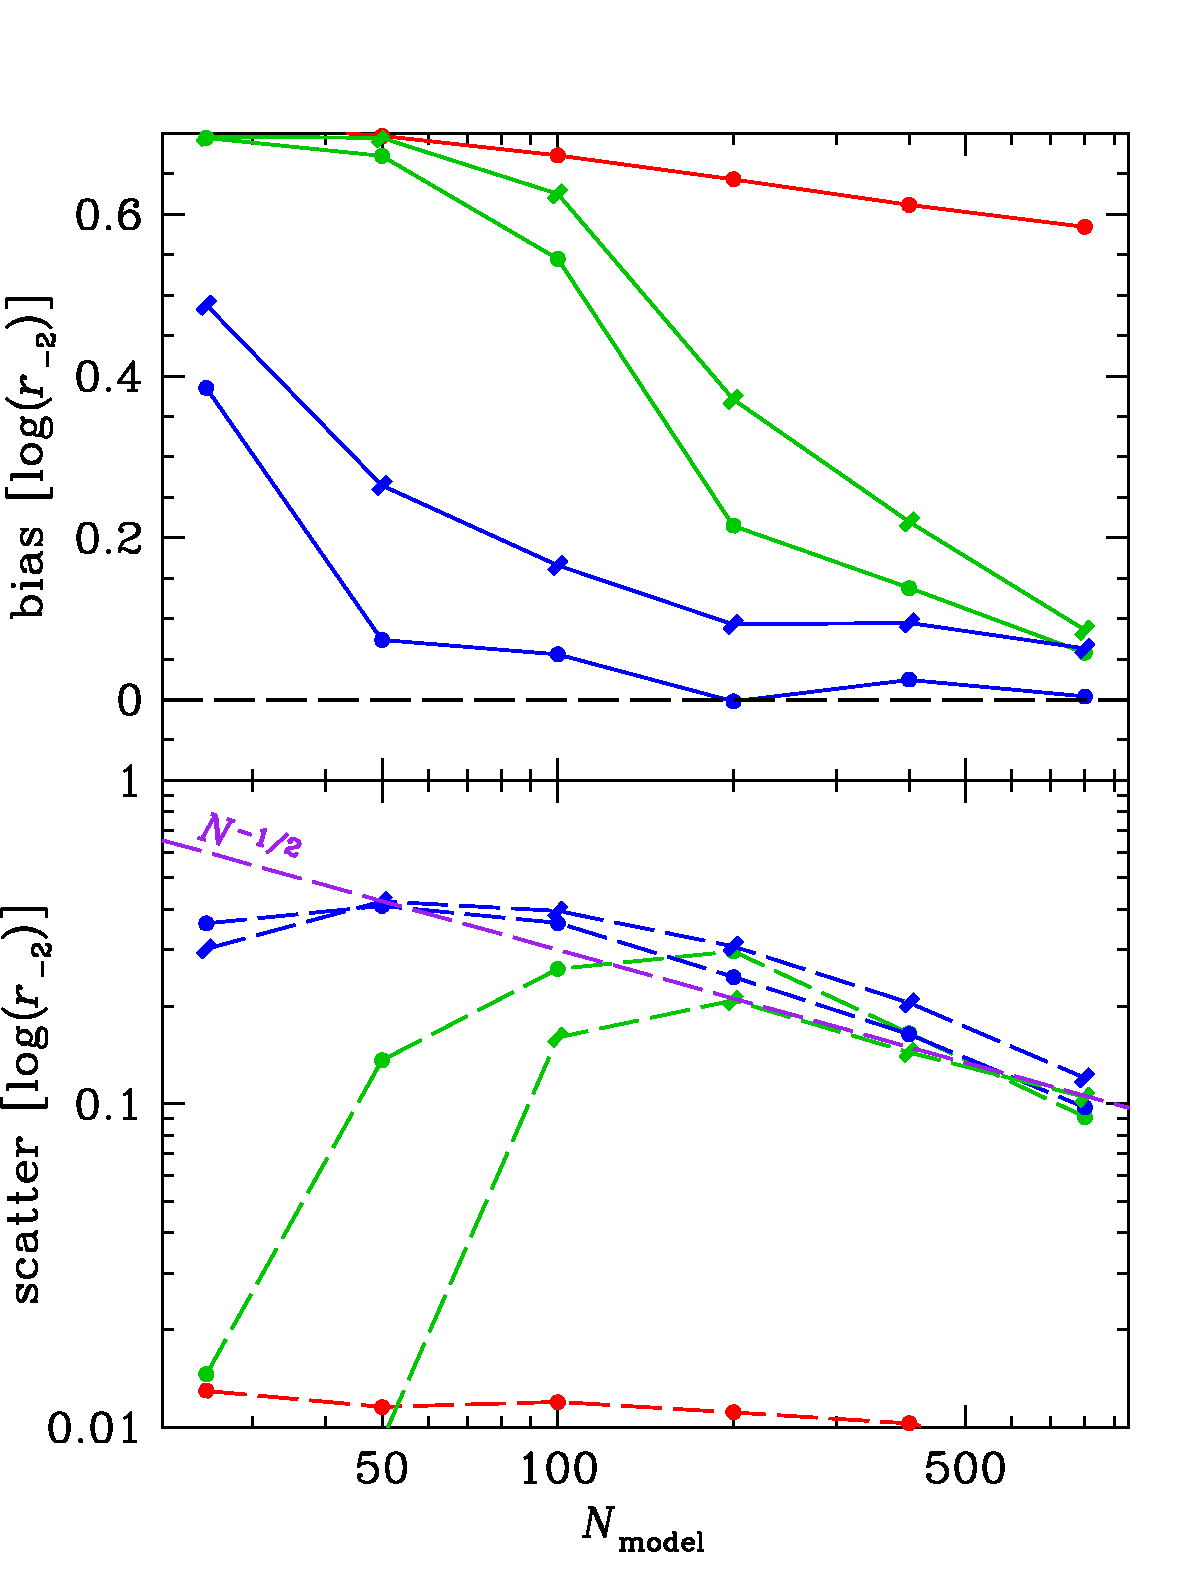
\includegraphics[scale=0.4]{loga_bias_circ.pdf}}
		\quad
		\centering
		\subfloat[]{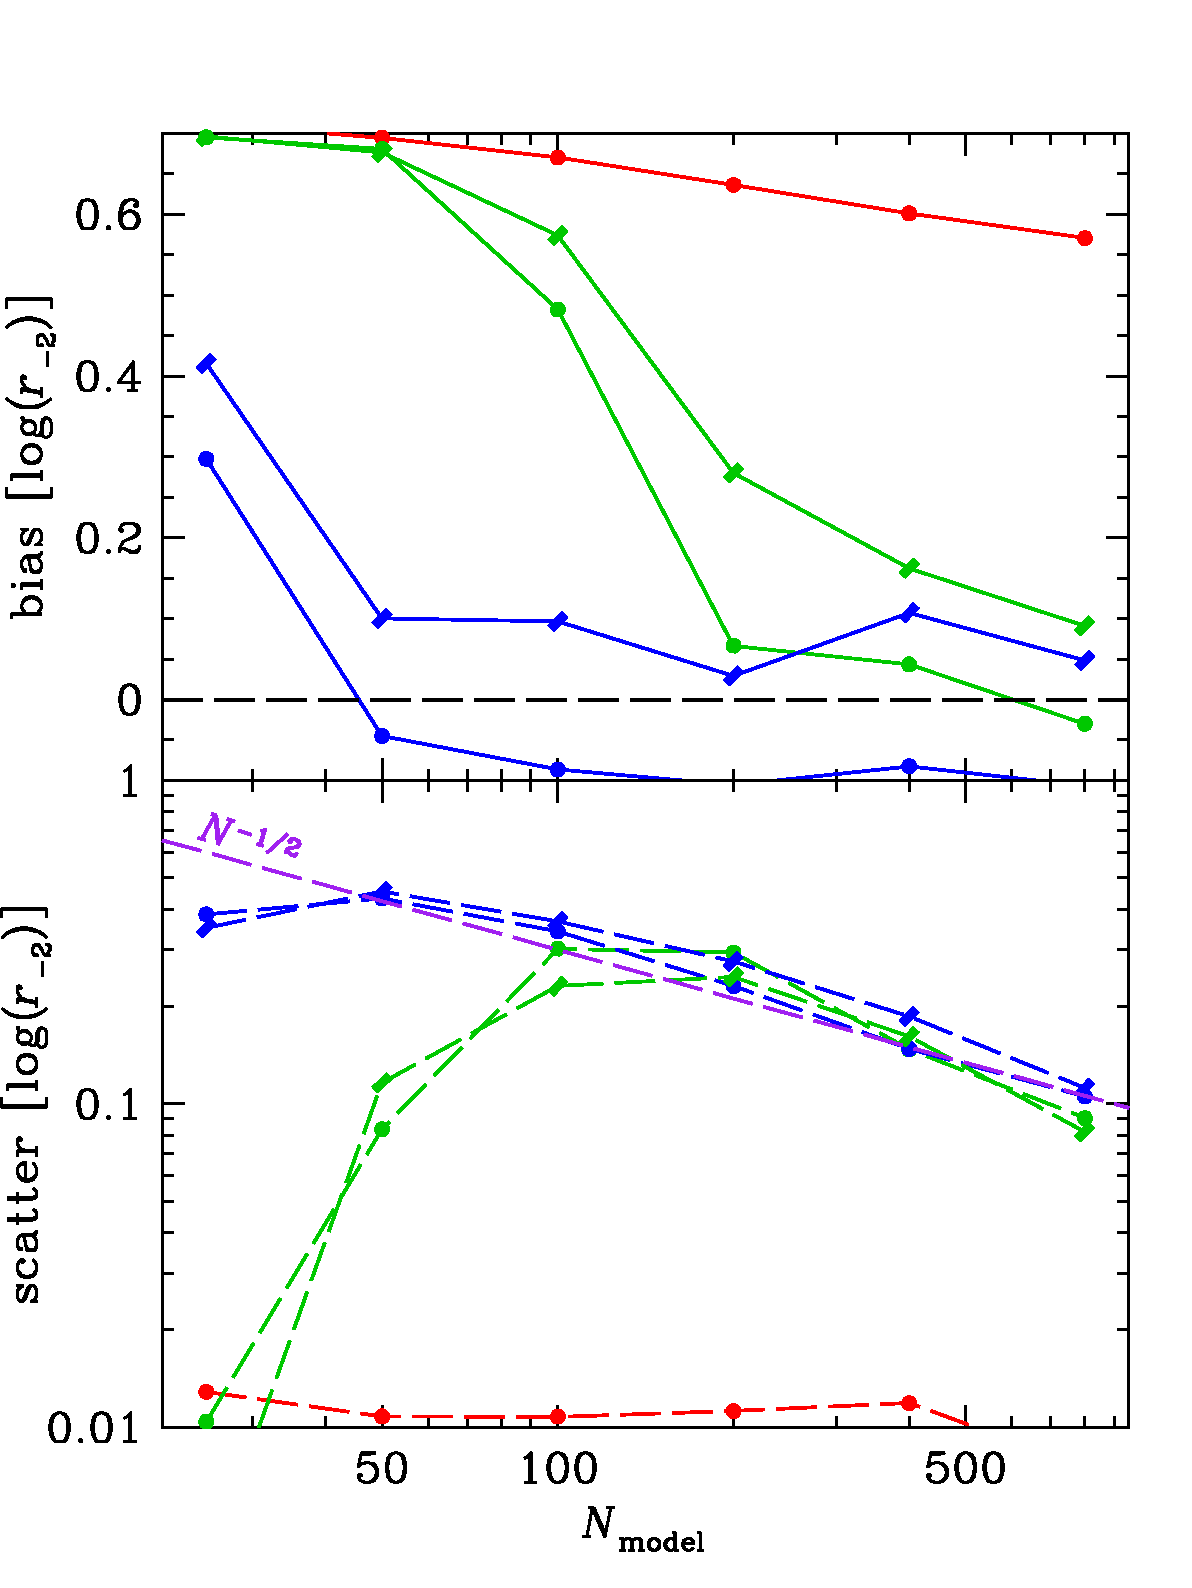
\includegraphics[scale=0.4]{loga_bias_ellip05.pdf}}
	\caption{Biais et dispersion en \textit{log scale radius} sur les mocks académiques avec à gauche un amas circulaire et à droite un amas d'ellipticité $0.5$. On trouve en vert, bleu et rouge respectivement les méthodes TNC, DE et séparation médiane. Les symboles elliptiques correspondent aux résultats du \textit{likelihood} en elliptique. DE se comporte globalement le mieux en terme de biais. La séparation médiane a un biais élevé mais comme attendu une dispersion très faible.}
	\label{fig:Median}
\end{figure}

  \section{Étude de la Séparation médiane}
    \subsection{Modélisation et calcul}
      Avant de commencer à étudier l'efficacité du code par maximum de vraisemblance, une alternative prometteuse semblait résider dans la séparation médiane entre les galaxies. En effet, si l'on a un amas sans fond constitué de $N$ galaxies, alors à $N$ plus élevé on a plus de résolution pour calculer la séparation médiane, ce qui en principe devrait donner intuitivement une loi en puissance $\Delta \propto r_{-2}^{\alpha}$, ou sous forme logarithmique $\log_{10} \Delta = \alpha \log_{10} (r_{-2}) + \beta$. \par
      En pratique on boucle dans le code sur $i,j$ avec $j<i$ et on calcule les $N(N-1)/2$ séparations $\Delta l_{kl} = \vert l_k - l_l \vert$. 
      On obtient alors la partie triangulaire supérieure d'une matrice symétrique sur laquelle on peut calculer la séparation médiane.
    \subsection{Analyse de la séparation médiane}
  	  La séparation médiane est comparée dans la Fig.\ref{fig:Median} avec DE et TNC. Celle-ci est grandement biaisée vers des valeurs positives. Comme attendu, on obtient une loi linéaire en log pour $N \gtrsim 50$ avec $\alpha \approx 1.7 \times 10^{-4}$ et $\beta \approx 0.8$. Étonnament, ces valeurs semblent être indépendantes de l'ellipticité de l'amas et changent peu pour des mocks amas+fond avec des valeurs de fond raisonnables. \par
  	  Le fait que la séparation médiane ne soit basée sur aucun modèle sous-jacent la rend peu sensible aux variations statistiques qui peuvent apparaître lors de la génération aléatoire des mocks. Conséquemment sa dispersion est très faible. De ce fait, la séparation médiane semble être une alternative intéressante si l'on arrive à corriger le biais qui semble systématique.
  	
  \newpage
  \section{Halo de matière noire : Profil NFW et surface de densité}
    On résume rapidement dans cette section les propriétés 3D et 2D des amas étudiés qui serviront dans le calcul du \textit{likelihood} dans la section \ref{sec:Likelihood}.
  
  \subsection{Profils NFW et NFW tronqués}
    Vers la fin des années 1990 Navarro, Frenck et White montrèrent à l'aide de simulations à N-corps que les halos de matière noire formés dans des cosmogonies de type CDM possèdent un profil de densité 3D NFW isotrope.
	Un tel profil est abondamment utilisé dans la littérature pour la modélisation de profil radial d'amas (modèle utilisé dans \cite{AMICO}). 
    Le profil NFW est généralement écrit sous la forme\cite{NFW1996}
    
    \begin{equation}
      \label{eq:NFW_profile}
      \frac{\rho(r)}{\rho_{crit}} = \frac{\delta_{char}}{(r/r_s) ( 1 + r / r_s)^2}
    \end{equation}
    
    Où $r_s$ représente le rayon de pente -2 et $\delta_{char}$ est une surdensité caractéristique que l'on relie au paramètre de concentration $c = r_s / r_v$ via la formule\cite{Mo_concentration}
    
    \begin{equation}
      \delta_{char} = \frac{200}{3} \frac{c^3}{\ln(1+c) - c / (1+c)}
    \end{equation}
    
	Un autre profil est parfois employé dans la littérature : le profil Einasto. Cependant nous nous restreindrons au profil NFW pour ce qui suit.
    
  \subsection{Densité surfacique projetée}
  \label{Densité_surfacique_projetée}
  	Les redshifts photométriques n'étant pas suffisamment précis pour nous fournir une information précise sur la distance des galaxies, le profil 3D n'a que peu d'intérêt en lui-même. 
    Les données traitées étant les positions projetées des galaxies sur le ciel, il nous faut non pas travailler avec la densité 3D, mais avec la densité surfacique projetée. Celle-ci est obtenue en intégrant le profil de densité le long de la ligne de visée
    
    \begin{equation}
      \Sigma (R) = \int_{\mathbb{R}} \rho (r) dz
    \end{equation}
    
    Où $r$ est le rayon 3D (ci-après rayon) et $z$ est la composante selon la ligne de visée. En notant $R$ le rayon dans le plan du ciel (ci-après rayon projeté), on peut réécrire cette dernière équation comme
    
    \begin{equation}
      \label{eq:Surface_density}
      \Sigma(R) = 2 \int _{R}^{\infty} \frac{r \rho (r) dr}{(r^2 - R^2)^{1/2}} 
    \end{equation}
    
    La solution analytique de cette équation donnée en Annexe \ref{Solutions analytiques de la densité de surface NFW/NFW tronqué} pour un profil NFW est utilisée par PROF-CL pour le calcul du \textit{likelihood}.
	Pour les données issus d'AMICO, les amas ne s'étendent pas jusqu'à l'infini mais sont en réalité tronqués jusqu'à un rayon $\sim r_{\rm{vir}}$. Cela signifie que Eq.\ref{eq:Surface_density} n'est plus correcte et qu'il faut effectuer le changement $\infty \rightarrow R_{\rm{trunc}}$ au niveau de la borne supérieure. Une solution analytique donnée en Annexe \ref{Solutions analytiques de la densité de surface NFW/NFW tronqué} est aussi utilisée par PROF-CL mais uniquement dans le but d'étudier les halos (cf. section \ref{sec:AMICO}).
	
	
	
  \begin{figure}
    \begin{minipage}{\textwidth}
    \vspace{-40pt}
    \centering
		\subfloat[]{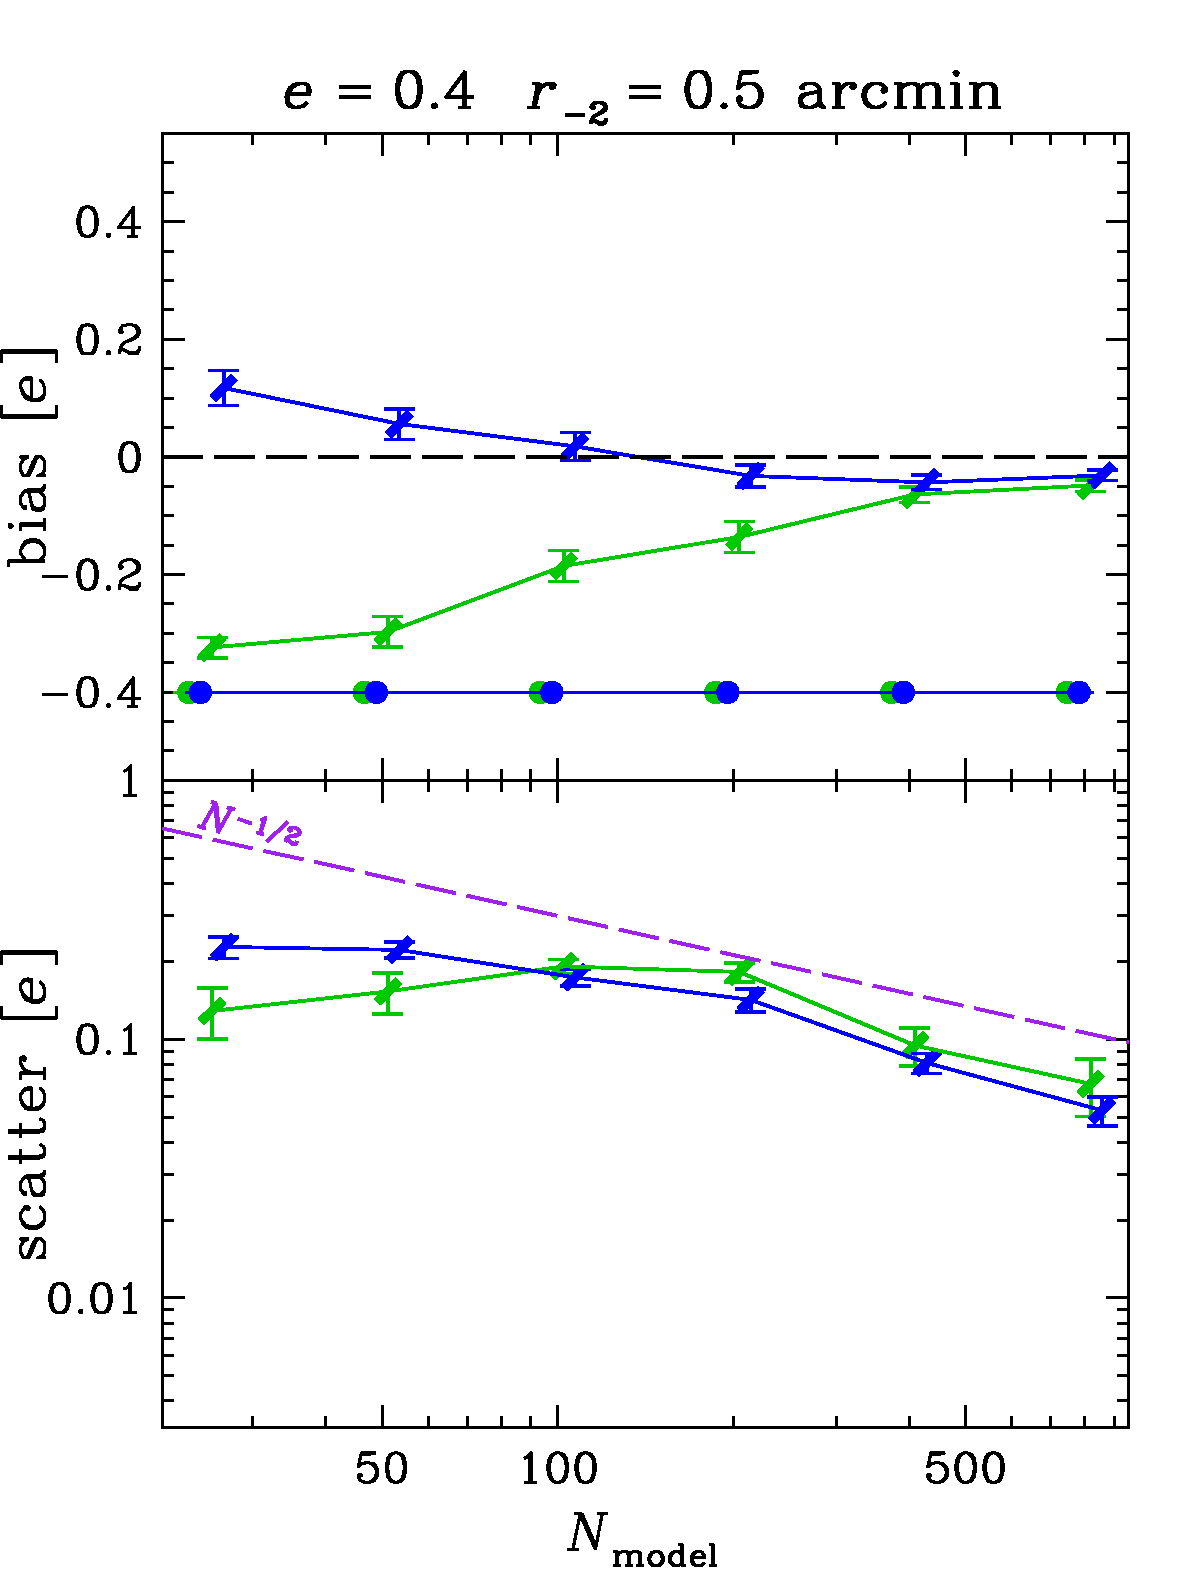
\includegraphics[scale=0.4]{ellipticity_bias_scatter_e4_a5.pdf}}
		\quad
		\centering
		\subfloat[]{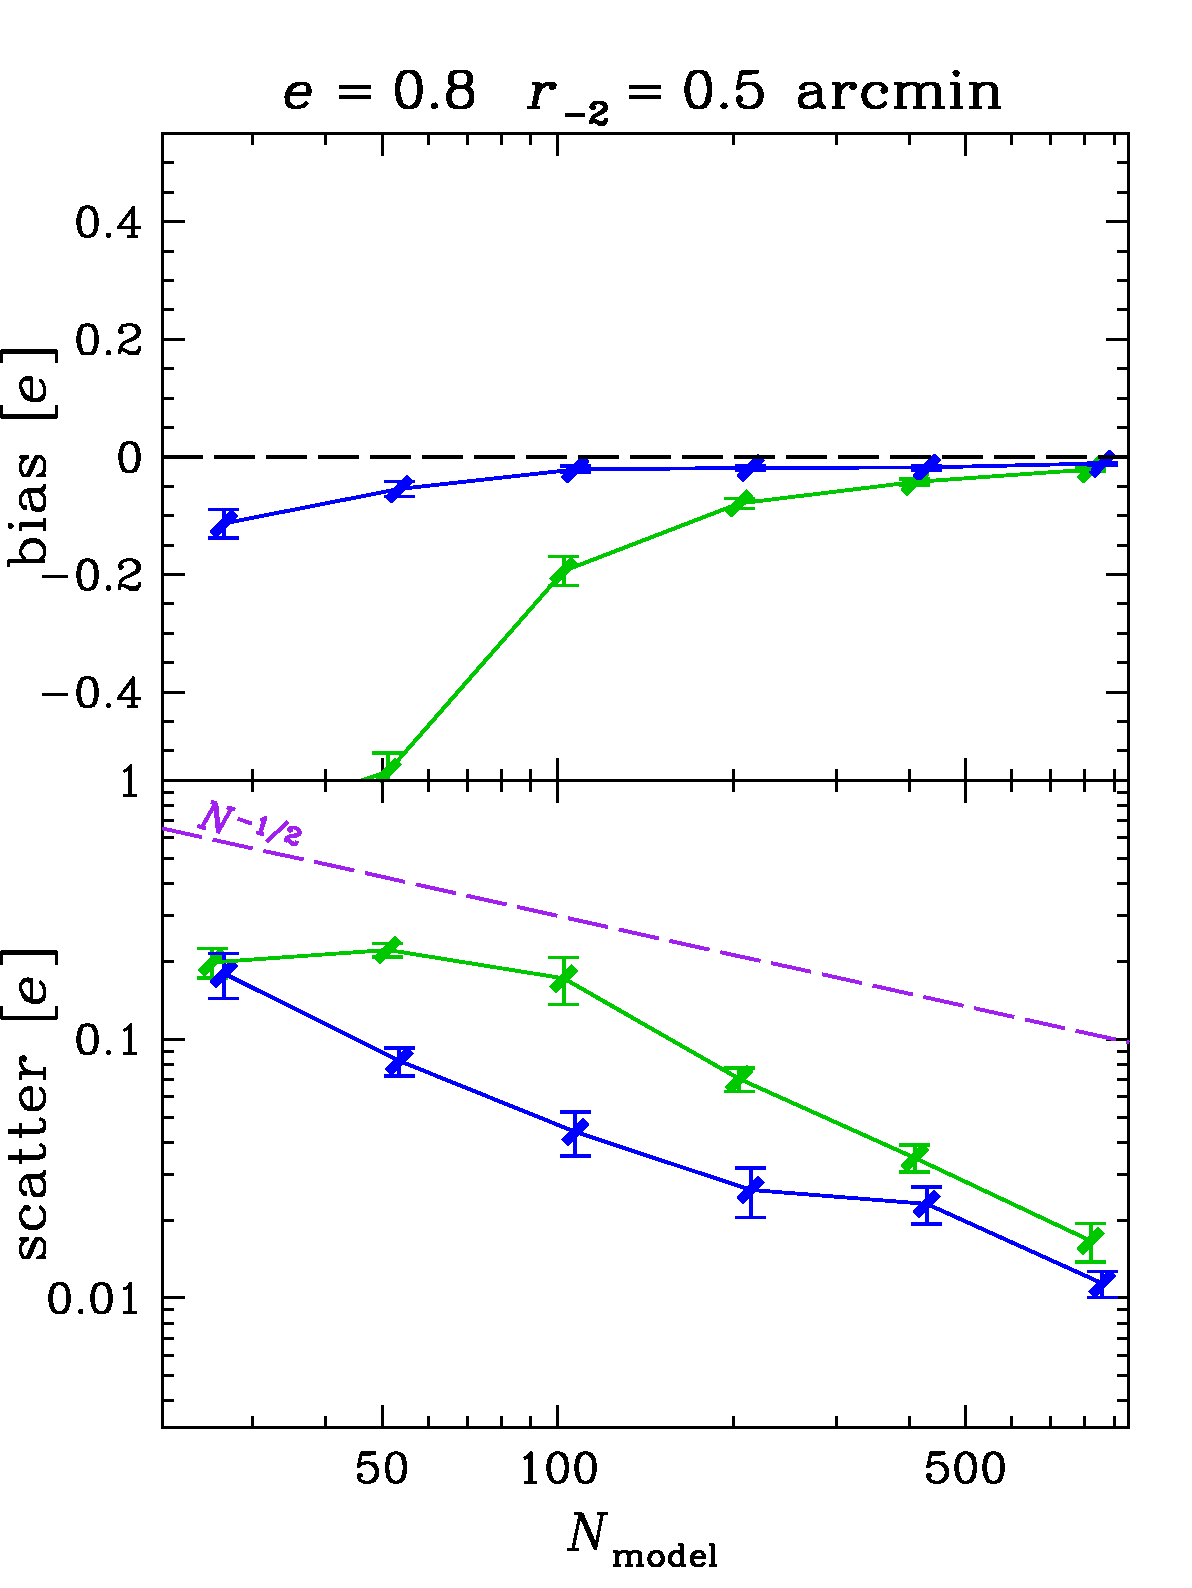
\includegraphics[scale=0.4]{ellipticity_bias_scatter_e8_a5.pdf}} \\
	  \subfloat[]{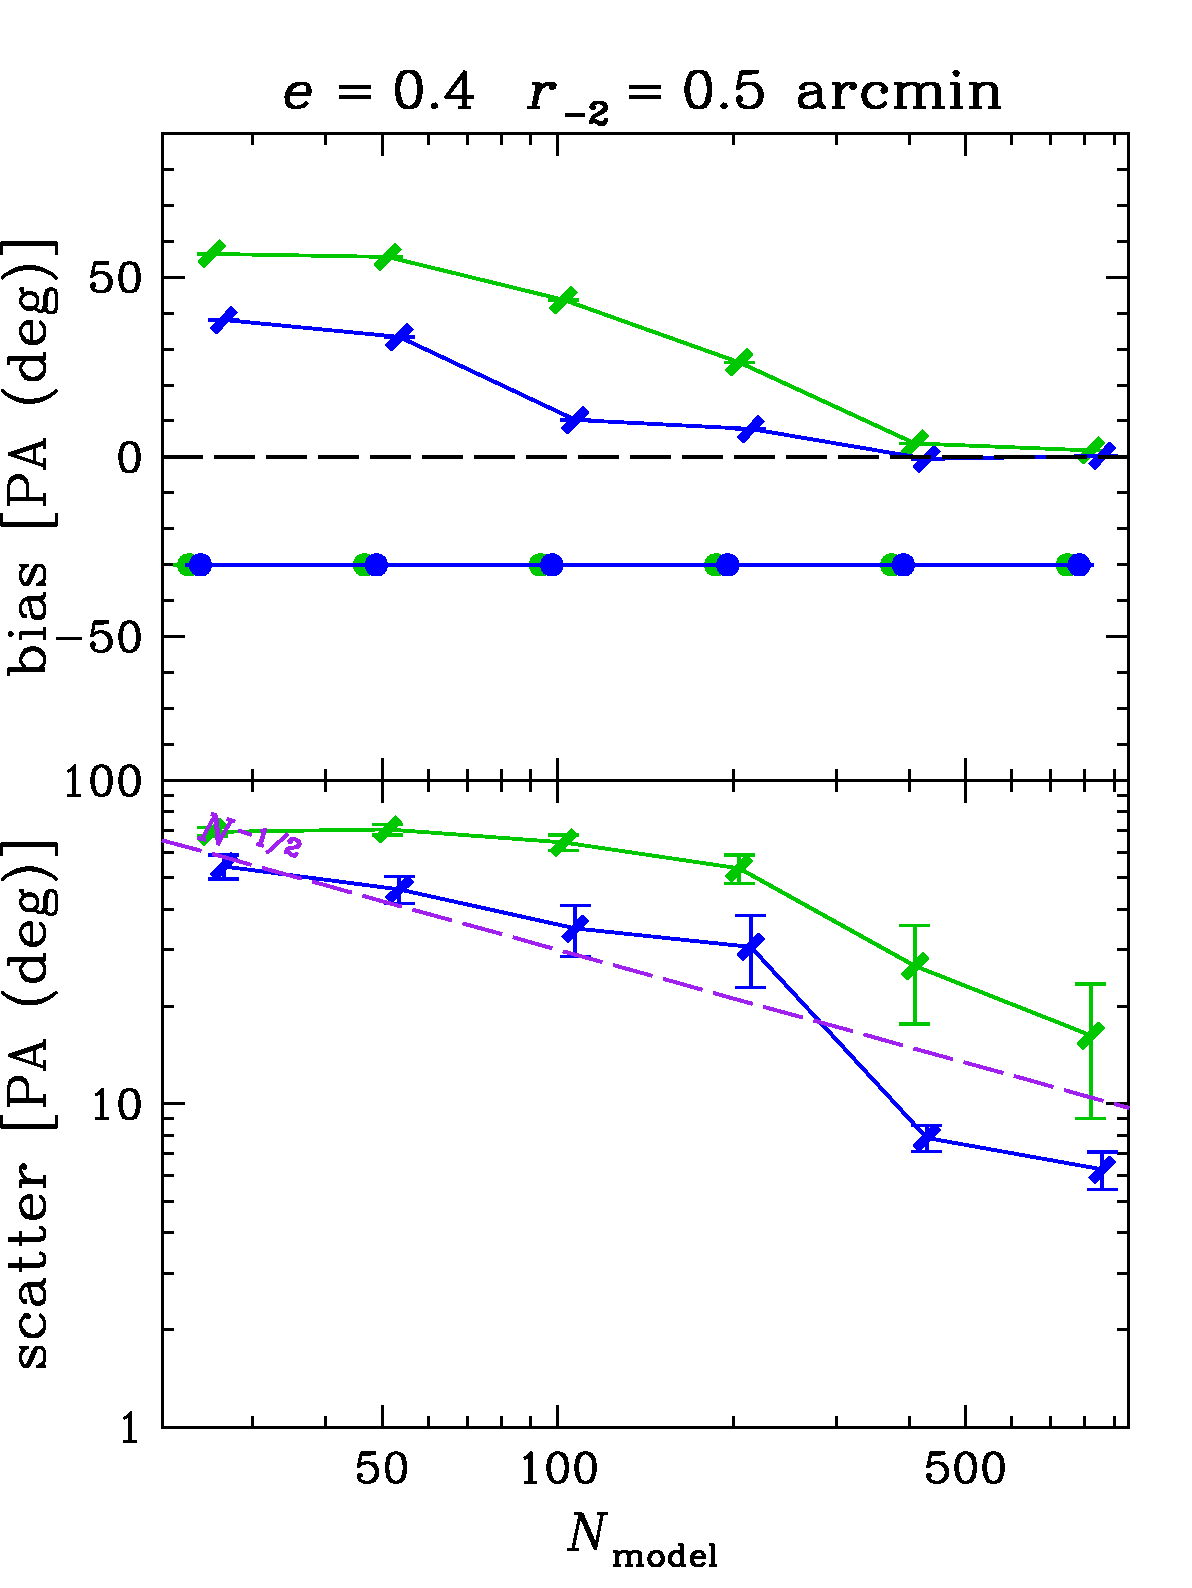
\includegraphics[scale=0.4]{PA_bias_scatter_e4_a5.pdf}}
		\quad
		\centering
		\subfloat[]{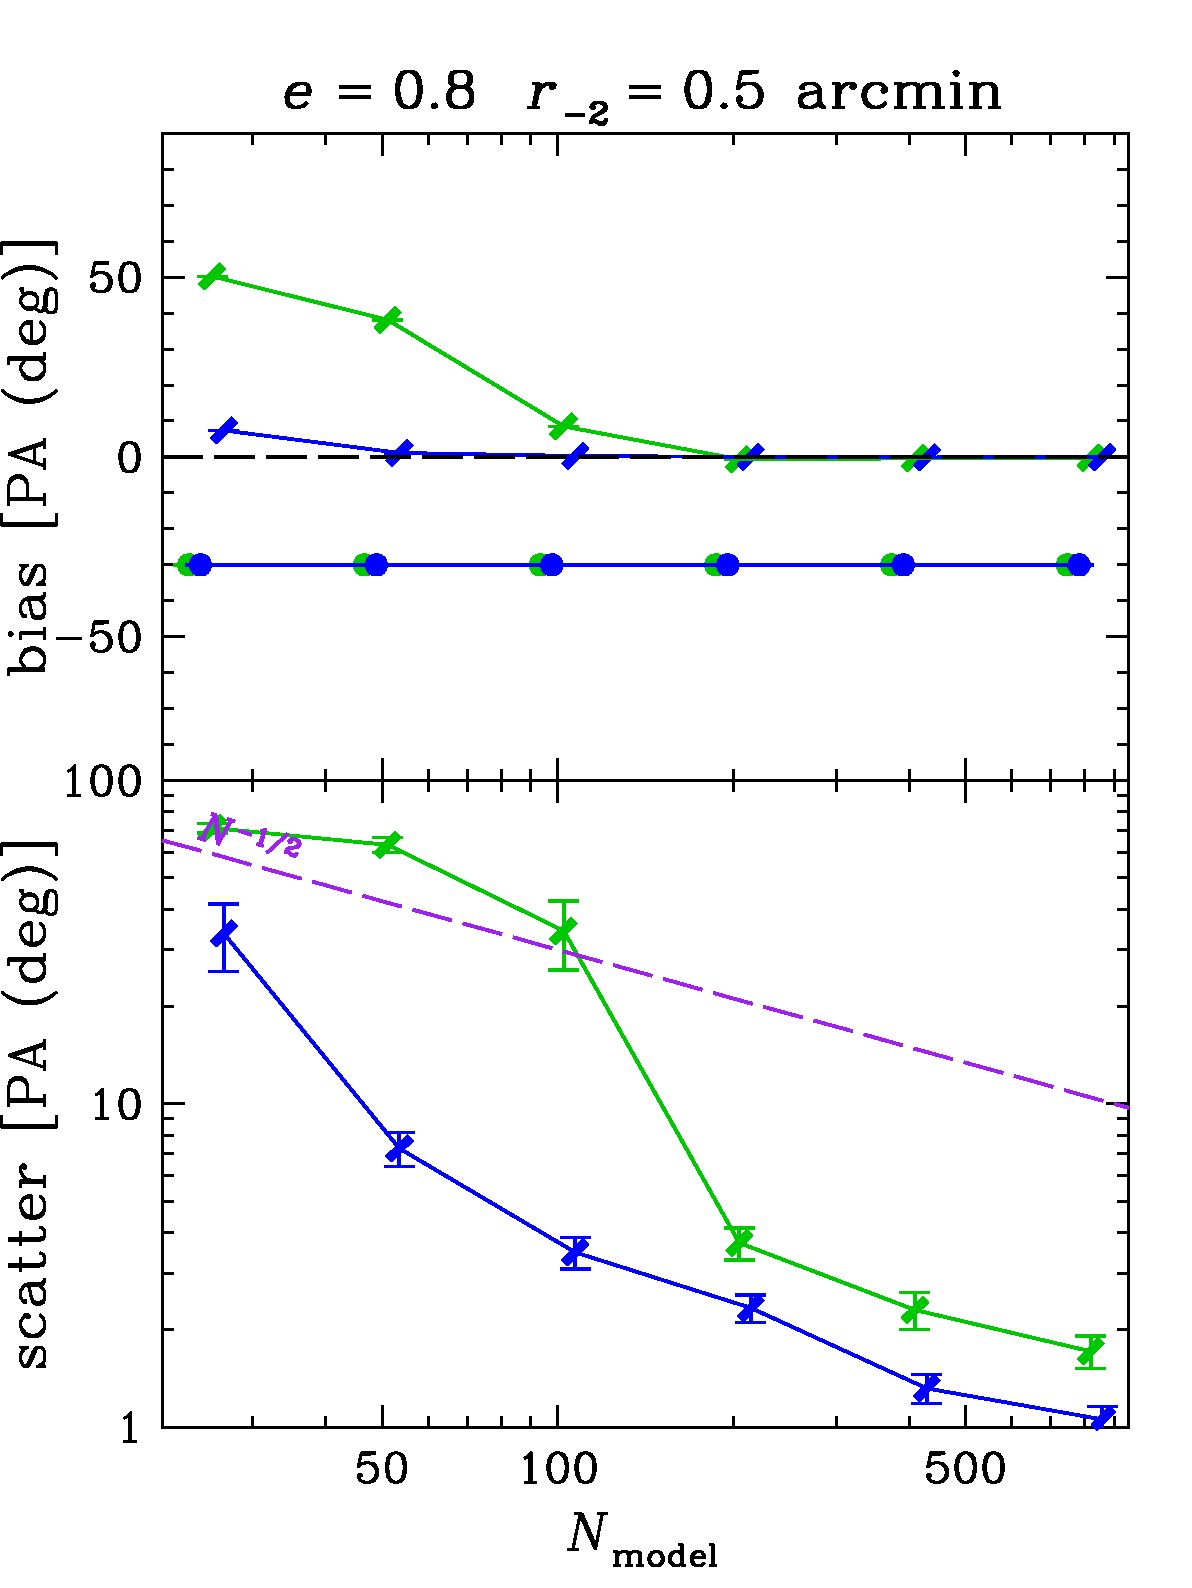
\includegraphics[scale=0.4]{PA_bias_scatter_e8_a5.pdf}}
	  \caption{Biais et dispersion en ellipticité et $PA$ pour deux types de mocks académiques elliptiques. Les couleurs et symboles sont similaires à celles de Fig.\ref{fig:Median}. Comme pour le \textit{log scale radius} DE obtient de meilleurs résultats que TNC en termes de biais et de dispersion. On remarque que le $PA$ est mieux trouvé à ellipticité élevée.}
	  \label{fig:Mocks}
	  \end{minipage}
  \end{figure}

	
	
	
	
	
  \newpage
  \section{Calcul du log-likelihood}
	PROFCL repose entièrement sur l'idée de trouver les meilleurs paramètres pour chaque halo par maximum de vraisemblance. Dans cette section on présente les équations utilisées par PROFCL et notamment celles développées lors du stage pour étudier des halos non-sphériques.  
  
  \label{sec:Likelihood}
  \subsection{Maximum de vraisemblance pour des amas de galaxies}
    Jusque dans les années 1980 l'unique méthode permettant de déterminer la densité surfacique projetée des amas était du \textit{binning-fitting}. Chaque image était découpée en anneaux de taille quelconque et le nombre de galaxies dans chaque anneau était compté. Sarazzin montra que ce type de méthode faisait apparaître des artefacts dans le rayon caractéristique des amas liés au choix de la taille des anneaux \cite{Sarazin1980}. Il proposa une méthode sans \textit{binning} basée sur le principe de maximum de vraisemblance.\par
    L'idée est d'assigner à chaque galaxie une probabilité de la trouver dans sa position étant donné le modèle considéré et les paramètres testés, puis de construire le \textit{likelihood} comme le produit de ces probabilités. Pour un ensemble de N galaxies de positions $ \lbrace \bm{X_i} = (x_i , y_i )_{1 < i < N} \rbrace $, en notant $\bm{\theta} = \lbrace \theta_i \rbrace $ l'ensemble des paramètres testés, on peut écrire le \textit{likelihood} comme
    
    \begin{equation}
      \label{eq:Likelihood}
      \mathscr{L} = \prod_{i=1}^N p( \bm{X_i} | \bm{\theta})
    \end{equation}
    
    Techniquement $p(\bm{X_i} | \bm{\theta})$ est une densité de probabilité normalisée à 1 telle que $p(\bm(X_i) | \bm \theta) d^2\bm{X}$ soit la probabilité de trouver la galaxie $i$ dans l'intervalle $[\bm{X_i} , \bm{X_i} + d\bm{X} ]$.\par 
    En pratique, puisqu'il est plus simple de minimiser une fonction que de la maximiser et que les probabilités considérées sont très faibles, on considère plutôt l'opposé du logarithme du \textit{likelihood} (\textit{log-likelihood})
    
    \begin{equation}
      \label{eq:Log_Likelihood}
      - \log \mathscr{L} = - \sum_{i=1}^N p (\bm{X_i} \in cluster) \log p (\bm{X_i} | \bm{\theta})
    \end{equation}
    
    où on a pris soin de pondérer chaque terme par la probabilité de trouver la galaxie dans l'amas correspondant. Celle-ci est fournie par AMICO mais pas par PZWav ou par les amas académiques. C'est pourquoi si la probabilité d'appartenance des galaxies n'est pas connue on la prendra  égale à 1.
    
    \subsection{Probabilité de position pour un amas sphérique}
    La probabilité d'appartenance d'une galaxie à un amas sphérique est relativement simple. Dans ce cas il n'est pas question d'ellipticité ou d'angle de position. Ainsi pour un modèle NFW, les paramètres se réduisent à $\bm{\theta} = \lbrace r_{-2} , \Sigma_{\rm{bg}} \rbrace$ et la probabilité s'écrit\cite{Mamon2010}
    \begin{equation}
      \label{eq:Prob_uv_circ}
      p(R | \bm{\theta}) =  \frac{2\pi R [ \Sigma (R) + \Sigma_{\rm{bg}} ]}{N_{\rm{tot}}}
    \end{equation}
    
    où $R$ représente le rayon projeté, $\Sigma$ est la densité surfacique du modèle et $N_{\rm{tot}}$ est le nombre total de galaxies dans l'amas qui, pour un amas dont l'extension angulaire va de $R_{min}$ à $R_{max}$, s'écrit
    \begin{equation}
      \begin{split}
        \label{eq:N_tot}
        N_{\rm{tot}} =  & \int_{R_{\rm{min}}}^{R_{\rm{max}}} 2 \pi R \Sigma_{\rm{tot}}(R) dR \\
                =  & N(r_{-2}) \Delta \tilde{N}_p + \pi \Sigma_{\rm{bg}} \Delta R^2
      \end{split}
    \end{equation}
    
    Où $\Sigma_{\rm{tot}}(R) = \Sigma (R) + \Sigma_{\rm{bg}}$ et où on a défini les quantités suivantes
      \begin{align*}
        N_{\rm{p}} (R) & = N(r_{-2}) \tilde{N}_{\rm{p}} \left ( R / r_{-2} \right ) \\
        \Delta R^2 & = R_{\rm{max}}^2 - R_{\rm{min}}^2 \\
        \Delta \tilde{N}_{\rm{p}} & = \tilde{N}_{\rm{p}} (R_{\rm{max}}/r_{-2}) - \tilde{N}_{\rm{p}} (R_{\rm{min}}/r_{-2})
      \end{align*}
      
	avec $N_{\rm{p}}(R)$ le nombre de galaxies projetées dans l'amas selon le modèle jusqu'à une distance $R$ et $\tilde{N_{\rm{p}}}$ l'équivalent adimensionné.
      
  Dans les faits, le terme $2\pi R$ dans Eq.\ref{eq:Prob_uv_circ} est constant et n'intervient pas dans la procédure de minimisation, on peut donc se permettre de le retirer du code (ce ne sera plus vrai dans le cas elliptique).\par
  Le facteur de normalisation $N(r_{-2})$ est quant à lui calculé via Eq.\ref{eq:N_tot} étant donné que l'on connaît à la fois le nombre total de galaxies appartenant à l'amas, son extension spatiale et la densité surfacique du fond testée.
  \subsection{Probabilité pour un amas elliptique}
  Dans le cas elliptique les paramètres sont $\bm{\theta} = \lbrace r_{-2} , \Sigma_{\rm{bg}} , e , PA \rbrace$. Eq.\ref{eq:Prob_uv_circ} n'est plus correcte car l'ellipticité doit être prise en compte. Puisqu'il n'existe pas de modèle elliptique pour la densité surfacique, l'idée va être de "circulariser" l'amas et d'exprimer la probabilité de trouver la galaxies dans cet amas circularisé.\par
	En pratique, on commence par tourner l'amas d'un angle $-PA$ puis on calcule les nouvelles coordonnées locales elliptiques $(u, v^{'})$  pour chaque galaxie comme décrit dans l'Annexe \ref{coord}.\par
	On peut à présent écrire la probabilité de positionnement de la galaxie de manière générale comme
	
	\begin{equation}
		\label{prob_ell}
		p( (u,v) | \bm{\theta}) = \frac{\Sigma_{\rm{tot}} (u,v)}{\iint_{\Gamma} \Sigma_{\rm{tot}} (u,v) \rm{du} \rm{dv} }
	\end{equation}
	
	où $\Gamma$ est le domaine d'intégration de l'amas circularisé tel que la probabilité soit normalisée à 1. Dans Eq.\ref{prob_ell} la densité surfacique totale peut s'écrire comme la somme du modèle et d'un fond constant 
	
	\begin{equation}
		\label{Density_surface_tot_ell}
		\Sigma_{\rm{tot}} (u,v) = \Sigma_{\rm{ell}} (u,v) + \Sigma_{\rm{bg}}	
	\end{equation}		

	Contrairement au cas circulaire, la densité surfacique du modèle n'est plus isotrope dans le système de coordonnées $(u,v)$. Cependant on peut la relier à une densité surfacique isotrope si on considère les coordonnées $(u, v^{'})$ via la relation
	
	\begin{equation}
		\label{Density_surface_link}
		\Sigma_{\rm{ell}} (u,v)= \frac{1}{1-e} \Sigma ( \mathscr{R} )
	\end{equation}
	
	En insérant Eq.\ref{Density_surface_tot_ell} dans le dénominateur de Eq.\ref{eq:Prob_uv_circ} on exprime le nombre total de galaxies
	
	\begin{equation}
		\label{eq:N_tot_ell}
		\begin{split}
			N_{\rm{tot}} & = \frac{1}{1-e} \iint_{\Gamma} \Sigma ( \mathscr{R} ) \rm{du} \rm{dv} + \pi \Delta R^2 \Sigma_{\rm{bg}} \\
			& = N(r_{-2}) [ \tilde{N}_{\rm{p}} (R_{\rm{max}}/r_{-2}, e) - \tilde{N}_{\rm{p}} (R_{\rm{min}}/r_{-2}, e) ] + \pi \Delta R^2 \Sigma_{\rm{bg}}
		\end{split}
	\end{equation}
	
	où on a défini les quantités suivantes
	
	\begin{align*}
		\tilde{N}_{\rm{p}} (R/r_{-2}, e) & = N_{\rm{p}}(R , e) / N(r_{-2}) \\
		N_{\rm{p}} (R, e) & = \frac{1}{1-e}  \int_{-R}^R \rm{du} \int_{- \sqrt{R^2 - u^2}}^{\sqrt{R^2 - u^2}} \Sigma_{\rm{ell}} ( \mathscr{R} ) \rm{dv}
	\end{align*}
	
	Comme pour le cas circulaire on obtient le facteur de normalisation $N(r_{-2})$ dans le cas elliptique via Eq.\ref{eq:N_tot_ell}.
	En combinant les résultats précédents on peut alors exprimer la probabilité de position d'une galaxie dans un amas sachant les paramètres $\bm{\theta}$ comme
	
	\begin{equation}
		p( (u,v) | \bm{\theta}) = \frac{1}{N_{\rm{tot}}} \left [ \frac{N(r_{-2})}{\pi r_{-2}^2 (1 -e)} \tilde{\Sigma}_{\rm{ell}} (\mathscr{R}/r_{-2}) + \Sigma_{\rm{bg}} \right ]
	\end{equation}
	
	
	
	
	
\newpage
\section{Amélioration des algorithmes de minimisation}

  \subsection{Gestion des limites}
  
    \begin{figure}
      \begin{minipage}[t]{0.48\textwidth}
      \vspace{0pt}

      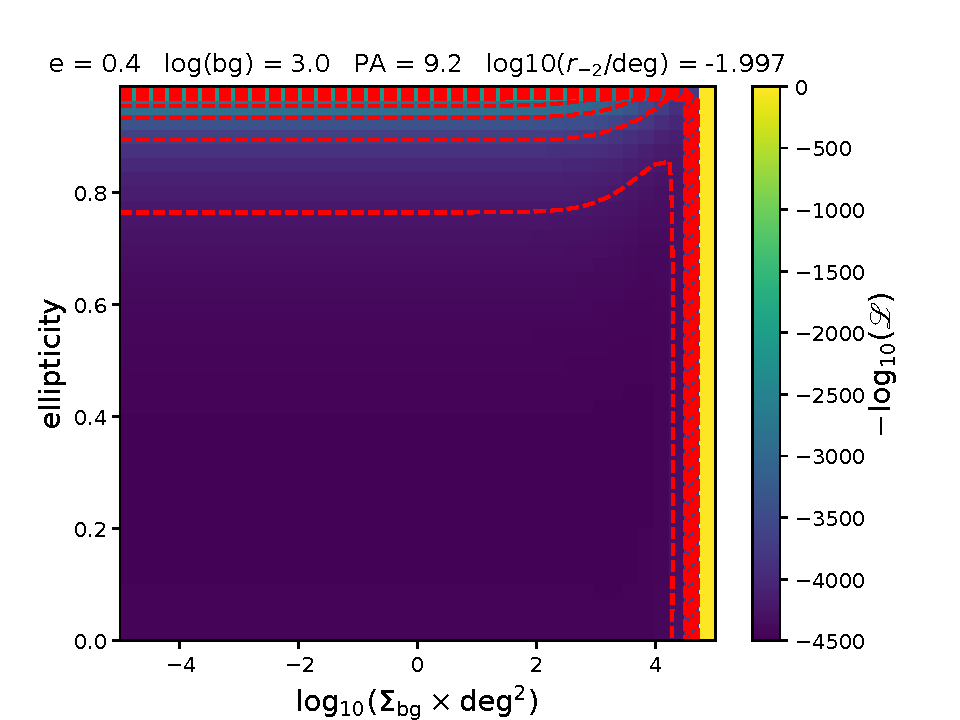
\includegraphics[width=\linewidth]{fixedPA_and_loga.pdf}
  		\caption{Portion de l'espace des paramètres à $PA$ et $r_{-2}$ fixés. On observe un "mur" au-delà de $\log_{10}(\Sigma_{\rm{bg}}) \sim 4.7$ lorsque la densité surfacique du fond sort des limites imposées. Le "mur" a été ramené à 0 pour des questions de visibilité. Les traits pointillés représentent les courbes d'iso-likelihood.}	  
  		\label{fig:Wall}
  	  \end{minipage}
	  \hfill
    \begin{minipage}[t]{0.48\textwidth}
      \vspace{0pt}
      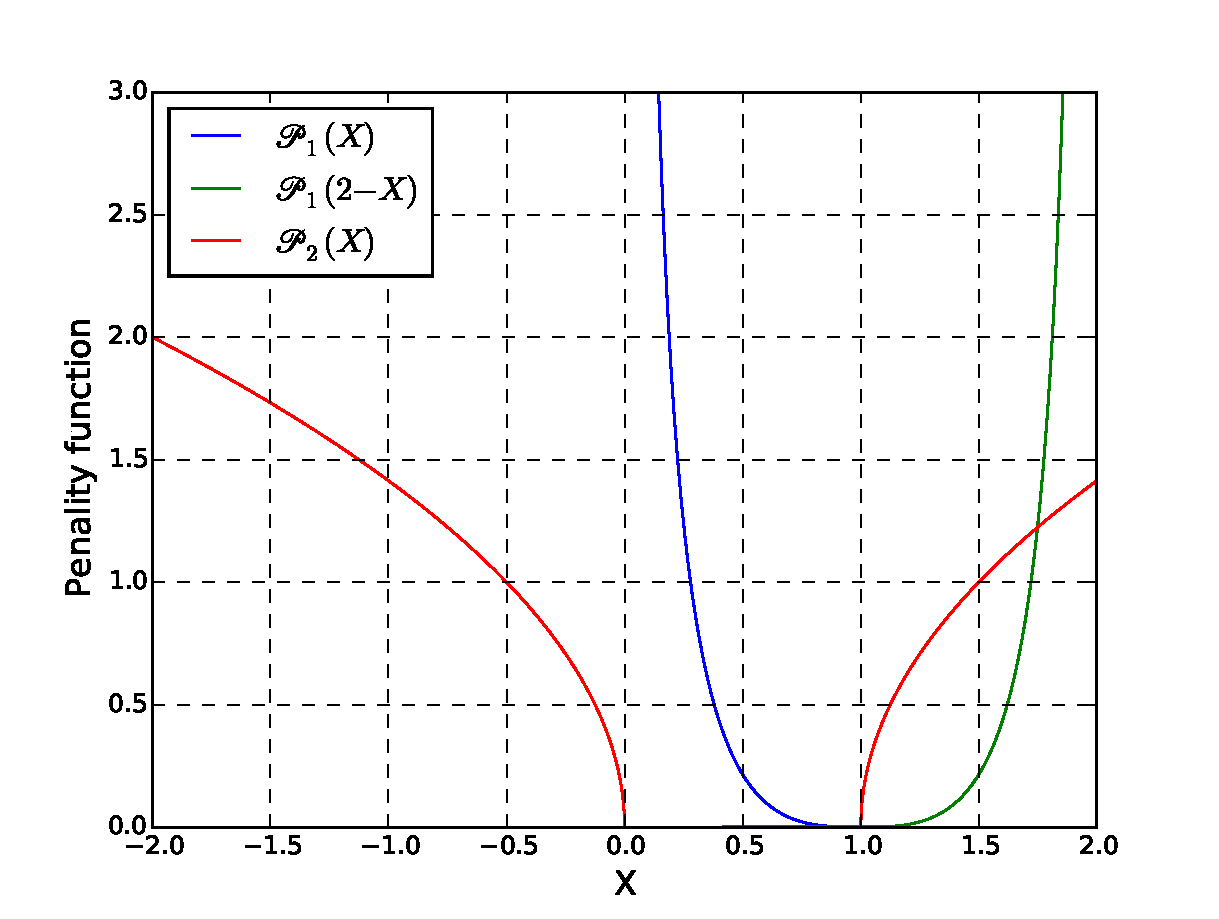
\includegraphics[width=\linewidth]{penalty.pdf}
  		\caption{Fonctions de pénalité intégrées dans PROFCL. En bleu la fonction pénalité n\degree 1 pour $X = x/x_{\rm{min}} < 1 $. En vert son symétrique par rapport à l'axe $X=1$ pour le cas $X = x/x_{\rm{max}} > 1$. En rouge la fonction de pénalité n\degree 2 avec $X = (x - x_{\rm{min}})/(x_{\rm{min}} - x_{\rm{max}})$.}
  	\end{minipage}
  	
  	\begin{minipage}[b]{\textwidth}
  	  \centering
		  \subfloat[]{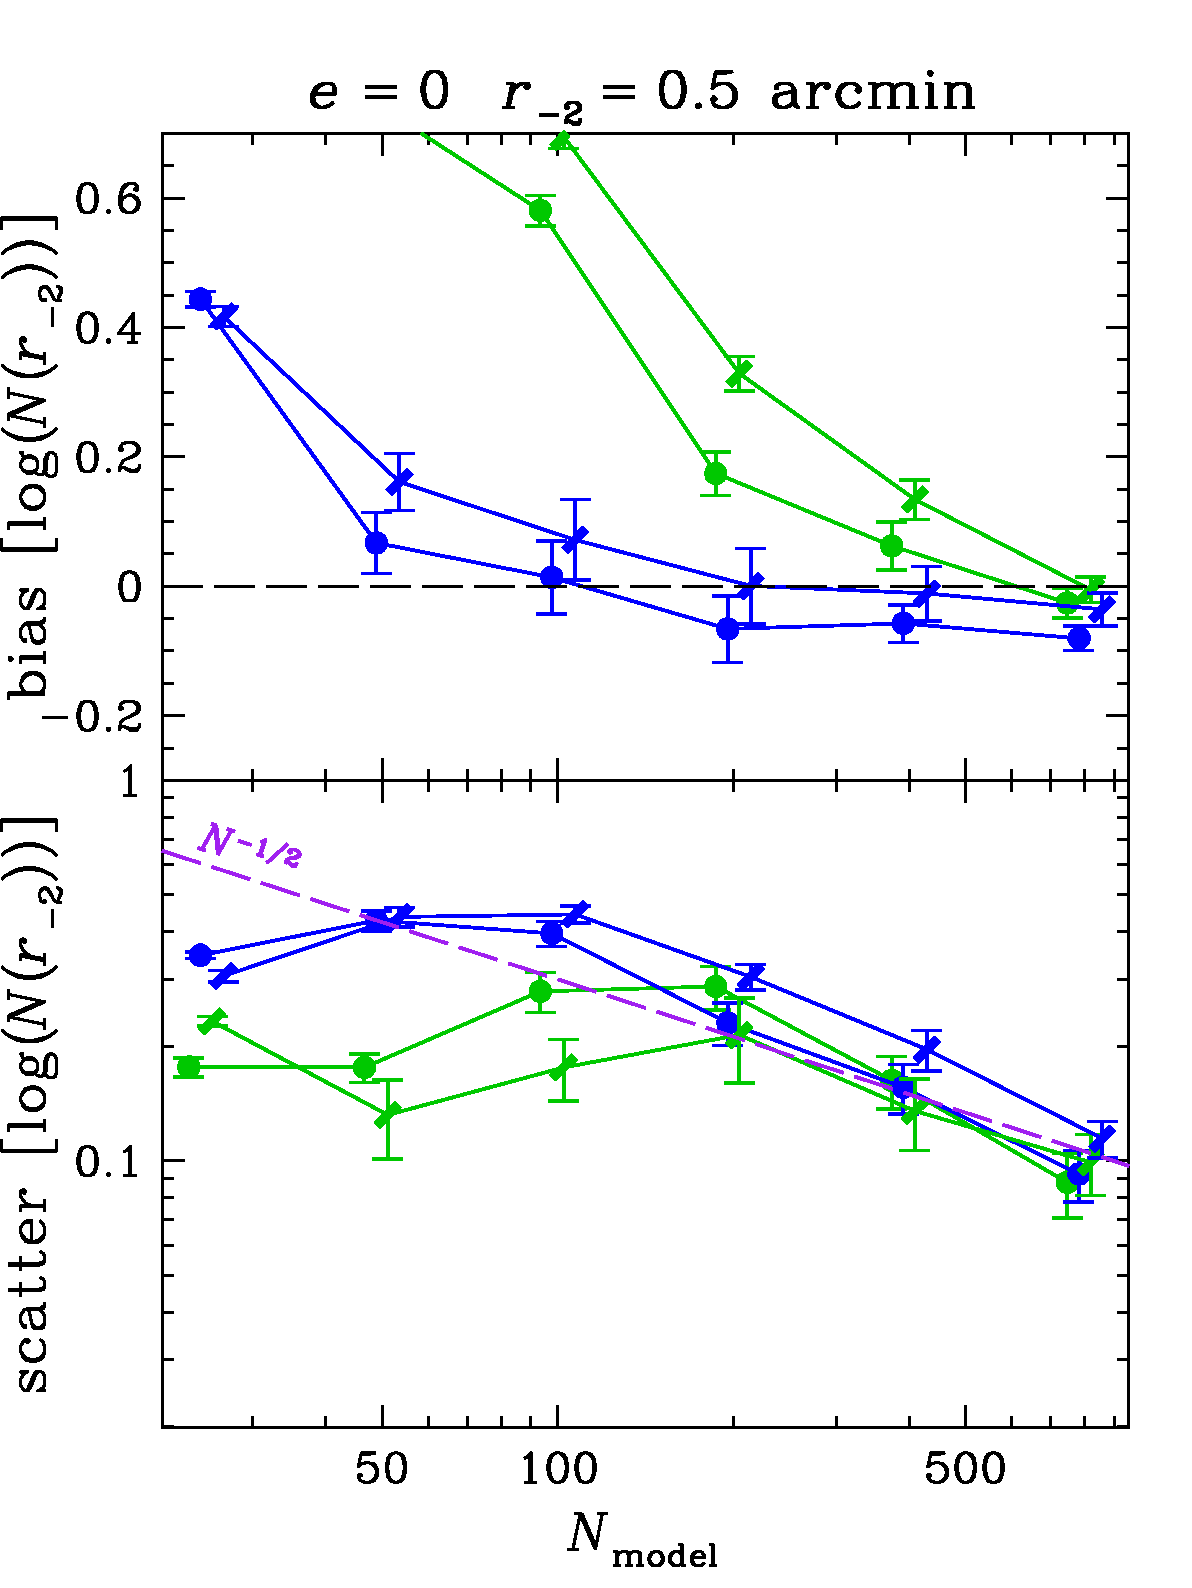
\includegraphics[scale=0.4]{logNofa_bias_scatter_e0_a5.pdf}}
		  \quad
		  \centering
		  \subfloat[]{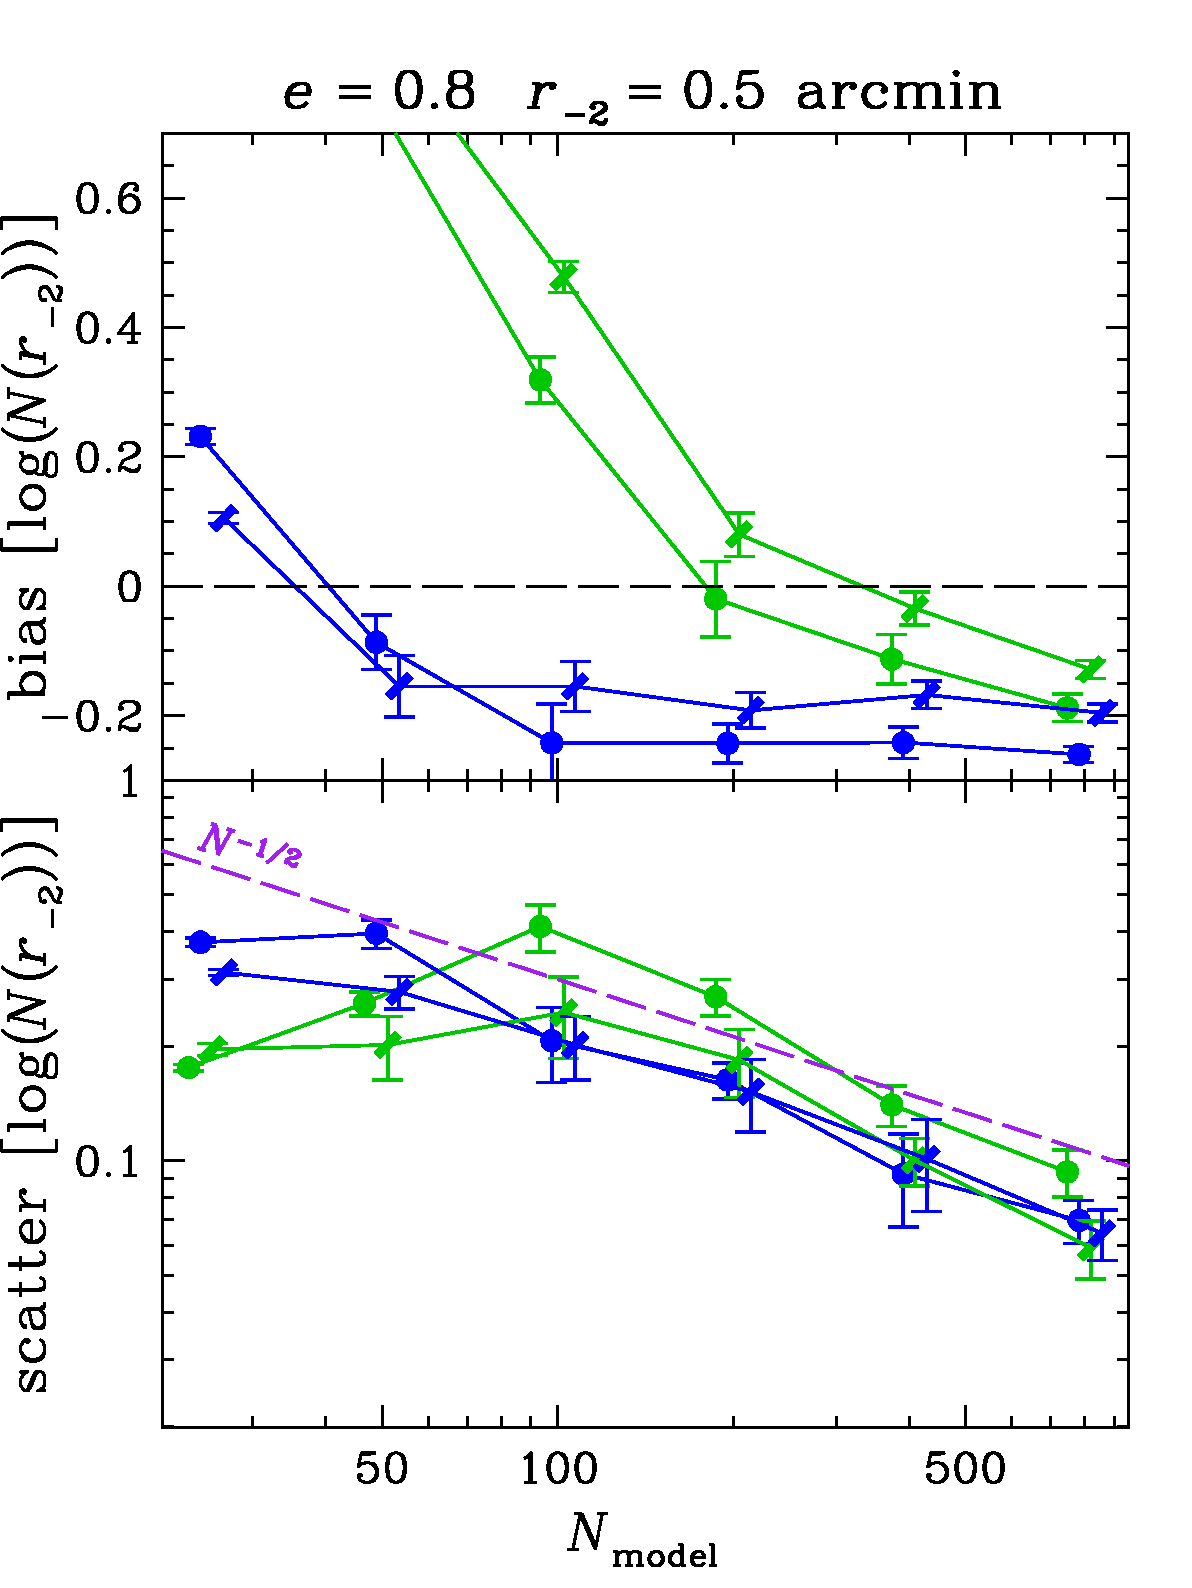
\includegraphics[scale=0.4]{logNofa_bias_scatter_e8_a5.pdf}}
		  \caption{Biais et dispersion en richesse sur les mocks académiques. La richesse est calulée via les relations Eq.\ref{eq:N_tot_ell} et Eq.\ref{eq:N_tot}. DE est en très bon accord pour le cas circulaire pour des richesses réelles $N \gtrsim 50$ et trouve de meilleurs résultats que TNC, en accord avec les résultats trouvés pour le \textit{log scale radius}. Les deux méthodes semblent converger vers un biais négatif pour de grandes ellipticités.}
  	\end{minipage}
  \end{figure}
  

	Certains algorithmes comme TNC ou BFGS prennent en compte la gestion des limites sur les paramètres de la fonction à minimiser. Dans ce cas il suffit de fournir pour chaque paramètre un intervalle qui va délimiter l'espace des paramètres à explorer. Au contraire certaines méthodes telles que DE ou NM peuvent en principe parcourir complètement l'espace des paramètres et donc, en principe, converger vers un minimum local pour des valeurs non-physiques.\par
	La solution qui avait été trouvée au début du stage était de tester les valeurs pour chaque paramètre et de retourner $- \log_{10} (\mathscr{L}) \sim 10^{30}$. En principe cette astuce devrait fonctionner pour DE car c'est un algorithme stochastique qui ira tester de nouvelles solutions ailleurs dans l'espace des paramètres. \par
	Pour NM, l'astuce ne fonctionne plus car l'algorithme va avoir tendance à rester localisé dans une même zone. Si l'algorithme est coincé dans un "mur" (cf. Fig.\ref{fig:Wall}), i.e. tous les sommets du simplex retournent $\sim 10^{30}$, l'algorithme ne saura plus dans quelle direction se déplacer. La solution à ce problème est d'ajouter une fonction qui va venir pénaliser le \textit{likelihood} de manière continue plutôt qu'une large valeur. 
	
	\subsection{Solutions mises en place}	
	Soit $\mathscr{P}$ une fonction pénalité et soit $x \in [x_{\rm{min}} , x_{\rm{max}}]$ un paramètre avec $x_{\rm{min}} ,x_{\rm{max}}$ les valeurs limites. Pénaliser le cas $x < x_{\rm{min}}$ revient à chercher une fonction avec les propriétés suivantes:
  \begin{itemize}
    \item $\mathscr{P} \xrightarrow{x \rightarrow -\infty} \infty$
    \item $\mathscr{P} (x_{\rm{min}}) = 0$
    \item $\left. \frac{d\mathscr{P}}{dx} \right | _{x=x_{\rm{min}}} = 0$
  \end{itemize}
  
  La dernière condition est ici pour assurer que la pénalité fonctionne aussi sur des méthodes de minimisation demandant des fonctions différentiables. Pour NM cette dernière n'est cependant pas importante. La première fonction pénalité qui fut mise en place dans PROF-CL est
  \begin{equation}
    \mathscr{P}_1(x) = 
    \begin{cases}    
      \mathcal{p} (X) & \mbox{si } X = x / x_{\rm{min}} < 1\\
      \mathcal{p} (2-X) & \mbox{si } X = x / x_{\rm{max}} > 1 \\
      0 & \mbox{sinon}
    \end{cases}
  \end{equation}
  
  où on a défini
  \begin{equation}
    \mathcal{p} (X) = 
      \frac{\pi}{2} (X-1) - \tan \left [ \frac{\pi}{2} (X+1) \right ]
  \end{equation}
  
  Bien que de classe $\mathscr{C}^1$, cette fonction n'adopte le comportement voulu que pour des valeurs de $X$ positives (i.e. $\mathscr{P} \xrightarrow{x \rightarrow 0} \infty$). Cela ne pose pas de problèmes, en principe, pour un algorithme comme NM car celui-ci n'ira jamais tester des valeurs négatives de $X$ si le paramètre initial n'est pas trop mauvais.\par
  Cependant l'algorithme Powell (intégré dans la dernière version mais peu testé) va quant à lui aller explorer l'espace des phases malgré un bon \textit{guess} de départ. Comme Powell ne requiert pas de fonction différentiable et pour éviter tout problème, on intègre dans le code une seconde fonction pénalité seulement $\mathscr{C}^0$ cette fois définie comme
  
  \begin{equation}
    \mathscr{P}_2(x) = 
    \begin{cases}    
      \sqrt{|\tilde{X}-1|} & \mbox{si } \tilde{X} > 1\\
      0 & \mbox{sinon}
    \end{cases}
  \end{equation}
  
  où $\tilde{X} = 2 | X - 1/2 |$ avec $X = (x - x_{\rm{min}})/(x_{\rm{min}} - x_{\rm{max}})$ permet d'assurer que les cas $x < x_{\rm{min}}$ et $x > x_{\rm{max}}$ sont traités de manière symétriques.
  
  
  \newpage
  \section{Performances du code sur les amas académiques}
  
    PROFCL a pu être testé sur plusieurs milliers de mocks académiques en circulaire et en elliptique, pour différentes valeurs de rayon caractéristique, d'ellipticité et de PA, avec et sans fond. Le fond jouant un rôle secondaire dans les résultats obtenus, on se concentrera sur le biais et la dispersion du \textit{log scale radius}, de l'ellipticité et du $PA$. Pour chaque jeu de paramètres $\bm{\theta} = \lbrace \log_{10} (r_{-2} , e , PA \rbrace$, 100 amas ont été générés aléatoirement suivant un profil NFW projeté isotrope par Monte-Carlo. De ces 100 amas, on a pu en tirer le biais moyen et la dispersion des paramètres. Les barres d'erreurs dans les graphes correspondent aux erreurs de Poisson $\epsilon = \delta / \sqrt{N}$ avec $N$ le nombre de mocks analysés statistiquement.
  
    Globalement DE obtient de meilleurs résultats que TNC. En moyenne, les deux méthodes convergent vers le résultat attendu à la fois en circulaire et en elliptique pour des richesses de l'ordre de $\gtrsim 500$. On peut cependant faire certaines remarques
  
    \begin{itemize}
      \item le \textit{log scale radius} est mieux trouvé dans le cas circulaire qu'elliptique pour les deux méthodes, y compris pour des amas d'ellipticité $\sim 0.5$
      \item DE calcule une très bonne richesse pour $N \gtrsim 50$ en moyenne mais la dispersion est large
      \item TNC donne de meilleurs résultats en terme d'ellipticité pour des amas circulaires
      \item DE sous-estime la richesse à large ellipticité
    \end{itemize}
  
    Le premier point n'est cependant plus vrai pour des ellipticités plus larges. Au delà de $e \sim 0.5$ on observe l'inverse avec un biais pour le cas elliptique qui converge très rapidement vers 0 tandis que le circulaire reste autour de $\sim -0.2$. \par
    Contrairement à TNC, la dispersion de DE peut être assez facilement corrigée dans la pratique. Cela est dû à l'aspect stochastique de l'algorithme qui va généralement obtenir un résultat excellent pour environs 5 lancers sur le même amas. Un moyen d'améliorer le scatter serait de diminuer la population des solutions dans l'espace des phases (cf. Section \ref{sec:Algo}) mais d'augmenter le nombre de lancers de DE. Bien que diminuer la population va réduire la convergence de l'algorithme, le fait de le lancer plusieurs fois va avoir pour effet de lui faire prendre des chemins différents dans l'espace des paramètres et donc d'augmenter le volume cherché. Une seconde manière d'améliorer la convergence et de réduire la dispersion serait de réutiliser à chaque nouveau lancer la meilleure solution des lancers précédents comme solution initiale.\par
    Le dernier point est étonnant étant donné que même le résultat en elliptique est biaisé négativement, et ceci malgré des résultats excellents en termes de \textit{log scale radius}, d'ellipticté et de $PA$. Un tel biais pourrait peut-être provenir d'une sur-évaluation de la densité surfacique du fond, ce qui entraînerait une diminution du nombre de galaxies dans la sphère.  
  
  
  
  
  
  \newpage
  \section{Étude de PROF-CL sur les amas AMICO}
  \label{sec:AMICO}
  
   \begin{wrapfigure}{l}{.5\linewidth}
     \vspace{-45pt}
     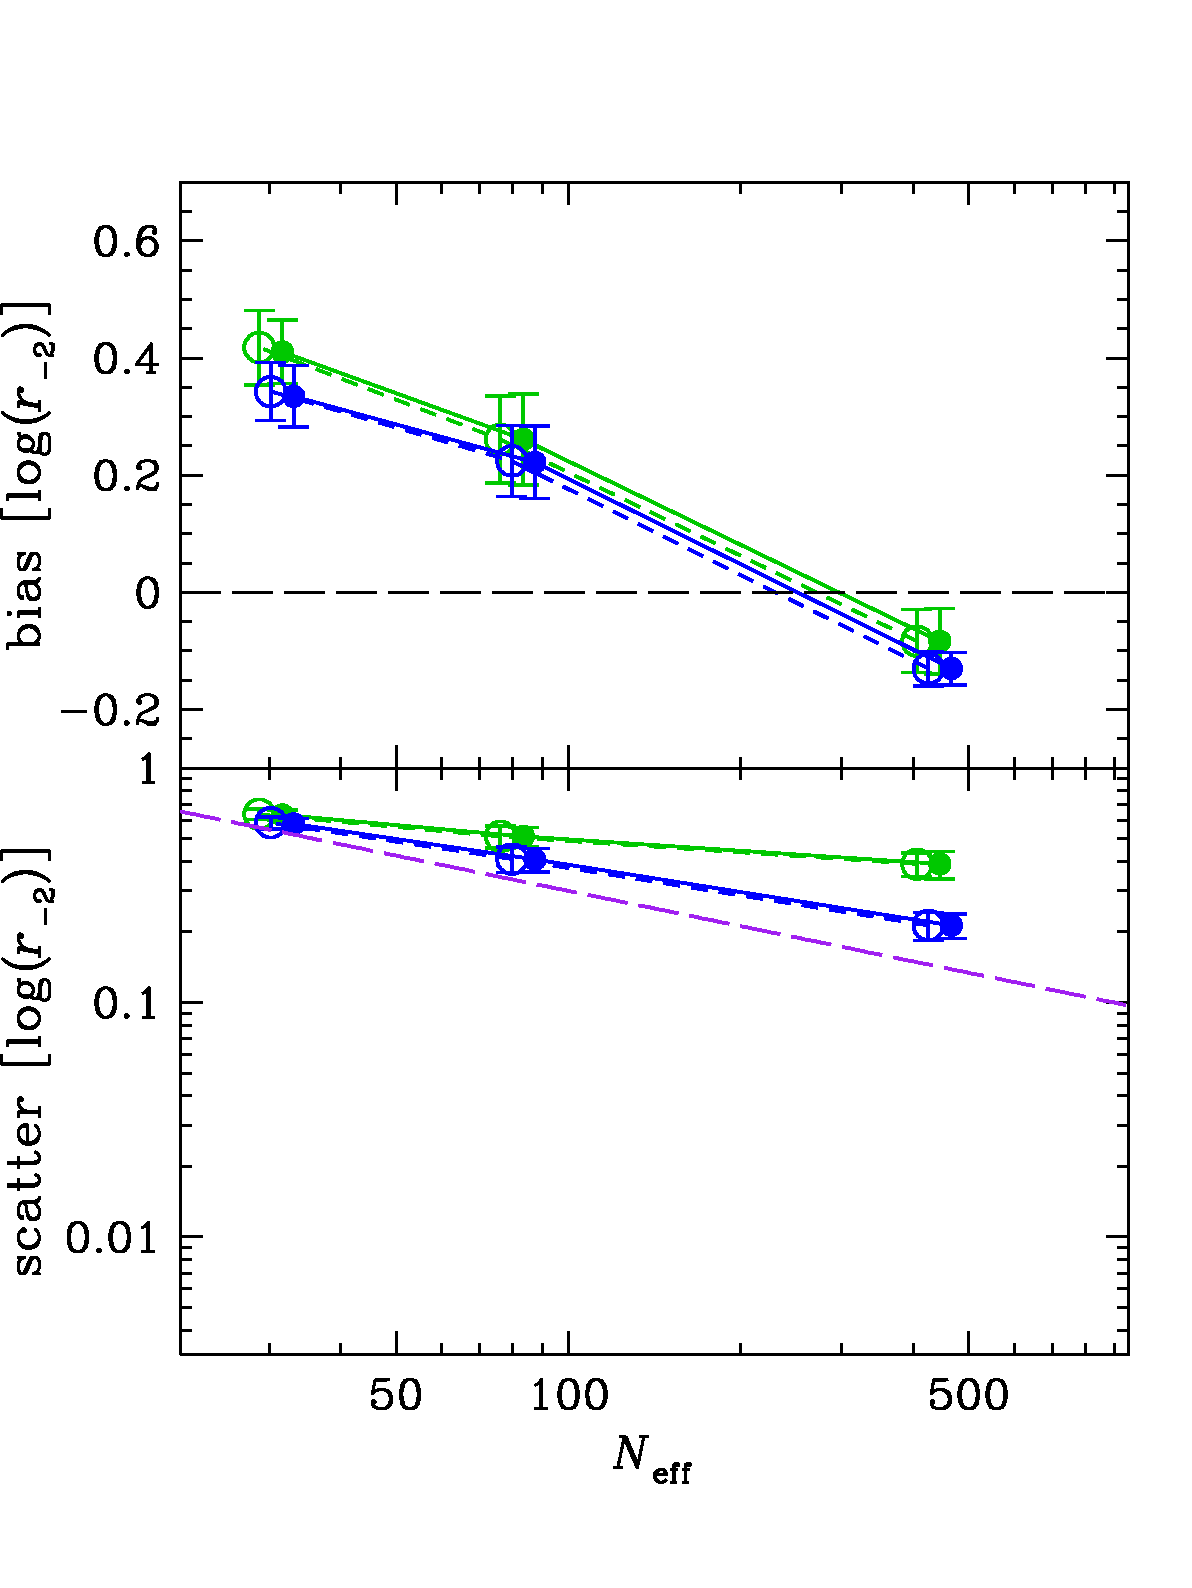
\includegraphics[width=\linewidth]{loga_bias_scatter_AMICO.pdf}
     \vspace{-40pt}
     \caption{Biais et dispersion en \textit{log scale radius} sur les amas trouvés par AMICO. Le biais est calculé par rapport au rayon trouvé par le NFW tronqué sur le halo correspondant. Pour éviter de donner trop de poids aux données à faible ratio $S/N$ les résultats ont été binnés dans trois intervalles de richesse $[20, 50]$, $[67, 150]$, $>200$. DE se comporte légèrement mieux que TNC en terme de biais et de dispersion.}
     \label{AMICO}
   \end{wrapfigure}
    
    \subsection{Méthodologie pour l'analyse de la performance de PROF-CL sur les données d'AMICO}
      Contrairement aux mocks académiques provenant des codes d'Artis ou de Mamon, les données fournies par AMICO ne permettent pas d'obtenir les paramètres réels des amas qui se sont formés dans la simulation. Le code AMICO, en plus de fournir les coordonnées des galaxies et leur probabilité, ainsi qu'un matching galaxies-amas, nous donne des informations supplémentaires au niveau des amas telles que leur richesse\footnote{La richesse calculée par AMICO n'est pas une mesure directe du nombre de galaxies dans l'amas mais plutôt une mesure de l'intensité des pics dans la carte 3D. Il est aussi possible d'estimer la richesse en sommant memberships des galaxies.}, leur redshift photométrique, l'erreur sur le redshift et le rapport $S/N$.\par
      Afin de pouvoir étudier la fiabilité de PROF-CL sur les amas d'AMICO, il nous faut donc déterminer la valeur "réelle" du rayon caractéristique directement sur la simulation. Une solution aurait été de fitter directement sur les données 3D un profil $\rho_{\rm{NFW}}$. Les données 3D n'étant pas disponibles, la solution trouvée fut de fitter directement sur les halos réels de la simulation un profil NFW tronqué projeté $\Sigma_{\rm{NFW}}^{\rm{trunc}} (R)$ et prendre comme rayon caractéristique "réel" la valeur retournée.\par
      Ce choix est dû au fait que la simulation semi-analytique place les galaxies dans les halos de matière noire jusqu'à une distance maximale de l'ordre de $2 r_{\rm{vir}}$ mais pas au-delà. Ce choix résulte dans un profil projeté sur le ciel tronqué au-delà d'un certain rayon $R_{\rm{trunc}}$ qui mène à des formules analytiques différentes de celles pour un profil non tronqué\cite{Mamon2010}. 
      
    \subsection{Matching des données AMICO et EUCLID}
      Avant de pouvoir étudier les performances de la dernière version de PROFCL sur les amas du code AMICO, il est nécessaire d'extraire des différents fichiers d'AMICO et d'EUCLID les informations intéressantes. AMICO fournit deux fichiers : détection.fits et association.fits. Le premier contient une liste d'identifiant des amas détectés ainsi que certaines de leurs propriétés. Le second fournit une corresondance entre les identifiants des amas, ceux des galaxies qui leur appartiennent et les \textit{memberships}. Il faut noter que les galaxies peuvent potentiellement appartenir à plus d'un amas.
      \subsubsection{Matching des données AMICO}
        Pour obtenir les positions des galaxies des amas, il est nécessaire d'aller faire correspondre les idenfiants des galaxies dans le fichier association avec le catalogue complet de $300\rm{deg^2}$ de la simulation. Le fichier complet faisant plus de $7\rm{GB}$, la difficulté principale a résidé dans le fait de faire correspondre coordonnées, identifiant et \textit{memberships} le plus efficacement possible.\par
        On a commencé par trier par identifiant croissant de galaxies le tableau de données du fichier de détection. Si on note $L_d$ la liste des identifiants triés du fichier de détection, alors on peut construire à partir de celle-ci une liste d'identifiants uniques $L_{\rm{ID}}$ de galaxies ainsi qu'une autre liste d'indices $L_i$ permettant de reconstruire la liste complète via la relation $L_d = L_{\rm{ID}} ( L_i)$. Une fois cette étape effectuée, on est en mesure de sélectionner dans le fichier complet l'ensemble des coordonnées correspondant aux identifiants dans $L_{\rm{ID}}$ et de trier le tableau obtenu par identifiants croissants. Il suffit alors d'appliquer $L_i$ à ce tableau pour reconstruire un tableau qui fait correspondre identifiants de galaxies, identifiants d'amas, membership et coordonnées.
      \subsubsection{Matching des données d'EUCLID}
        Pour pouvoir étudier les performances de PROFCL avec AMICO il nous faut aussi pouvoir fitter un profil NFW tronqué directement sur les halos issus de la simulation. La fragmentation et l'over-merging\footnote{Fraction d'amas associés à plus d'un halo} assez élevés d'AMICO vont avoir tendance à ce que l'algorithme décompose les halos en plusieurs amas ou au contraire associe à un amas plusieurs halos. On s'attend donc à ce que les galaxies associées aux halos ne soient pas les mêmes que celles associées aux amas.\par
        Le matching dans le cas des halos est légèrement plus complexe. AMICO fournit un fichier .fits fournissant un lien entre amas détectés et halos associés. Un amas peut apparaître plusieurs fois dans le fichier s'il y a over-merging et un halo de même s'il y a de la fragmentation. Puisque qu'un amas peut être lié à plusieurs halos, on n'est pas en mesure dans certains cas de savoir à quel halo comparer l'amas. Dans ce cas on choisit le halo le plus proche de l'amas comme point de comparaison. On peut ainsi construire un tableau liant bijectivement amas détecté et halo issu de la simulation.\newline
        Une fois le matching amas-halo effectué il faut lier galaxies et halos via un cinquième fichier .fits équivalent au catalogue complet à l'exception que cette fois à chaque galaxie ne correspond qu'un seul halo. Si l'on appelle $L_h$ la liste des halos bijectivement associée à celle des amas ($L_a$), lier les coordonnées des galaxies aux halos revient à lier celles-ci à $L_a$ dans un premier temps, puis à $L_h$ via la relation $L_h \leftrightarrow L_a$.     
         
    \subsection{Analyse des performances du code sur les amas d'AMICO}
      Pour analyser PROFCL sur les amas d'AMICO on a sélectionné un ensemble de 1000 amas sur lesquels environs 550 ont pu être associés à des halos. Les amas ont été choisis selon leur \textit{rank} croissant, c'est-à-dire selon leur rapport signal-bruit décroissant, dans 10 intervalles de 100 amas de telle sorte à ce que les résultats obtenus soient aussi valables pour des amas très massifs et bien résolus que pour des amas peu riches avec une forte composante de bruit. Par manque de temps les amas AMICO n'ont pu être analysés qu'en NFW circulaire seulement et les halos correspondant en NFW tronqué circulaire. \par
      Les résultats sur le \textit{log scale radius} sont représentés en Fig.\ref{AMICO}. Comme pour les mocks académiques, DE donne de meilleurs résultats que TNC mais la différence est bien moins prononcée. Les biais ont des valeurs similaires à ceux des mocks académiques. La dispersion décroît moins rapidement pour les amas AMICO ce qui est d'une part dû au binning effectué et d'autre part à la grande diversité des amas (cf. Annexe \ref{Amas}). Ne connaissant pas l'ellipticité réelle des amas, on n'est pas en mesure de pouvoir séparer amas circulaires et elliptiques de manière automatique ce qui induit nécessairement une dispersion plus grande. À cela vient s'ajouter le fait que la fragmentation va avoir tendance à induire un biais négatif dans le rayon caractéristique tandis que \textit{l'overmerging} va introduire une incertitude dans le choix de l'amas sur lequel effectuer la comparaison ce qui peut en principe introduire un nouveau biais. Enfin, il est important de noter que malgré la grande efficacité d'AMICO a détecter des sous-structures de résolution plus faible dans les données issues de la simulation par OF, on remarque aisément que dans un certain nombre de cas non-négligeable des sous-structures non détectées par AMICO apparaissent dans les amas. Si ces structures sont bien indépendantes les unes des autres cela va nécessairement introduire statistiquement un biais positif pour le rayon. \par
    Compte des origines des biais citées ci-dessus, les résultats obtenus sont assez encourageant bien que des statistiques plus poussées sur plus d'amas en prenant en compte l'ellipticité sont nécessaires. 
    
    \newpage
    \section{Conclusion et ouverture}
      Pendant ce stage, j'ai pu participer à l'amélioration et à l'analyse des performances du code - toujours en développement - PROFCL qui cherche à déterminer les caractéristiques d'amas de galaxies à partir des futures données de la mission EUCLID. Ces deux mois très enrichissants furent un moyen d'étendre mes connaissances dans des domaines variés, autant au sujet des simulations cosmologiques à N-corps et des codes semi-analytiques associés que sur les amas de galaxies de manière générale et de leurs propriétés en passant par tout un ensemble de techniques et algorithmes parmi lesquels certains que je n'ai pu détailler, voir mentionner (spline cubiques, bootstraps, etc). \newline\par

      Le code dans sa version actuelle est fonctionnel à la fois sur les mocks académiques et sur les données AMICO. Les difficultés majeures qui ont pu être rencontrées pendant le stage (séparation médiane non fonctionnelle, gestion des données AMICO, équation de probabilité de position non valable en elliptique, etc) ont pu être entièrement résolues.\par
    Certaines difficultés rencontrées pendant le stage ou certaines parties du code sur lesquelles j'ai pu travailler n'ont pas été mentionnées dans ce rapport soit car elle ne représentent pas la majorité du travail effectué, soit car leur implémentation n'a pas fourni de résultats significatifs sur les performances du code et n'ont donc pas été étudié suffisament en profondeur. Qui plus est certaines fonctionnalités supplémentaires comme la possibilité de rajouter le rencentrage comme paramètre supplémentaire dans PROFCL (en réalité 2 paramètres $RA_{\rm{cen}}$ et $Dec_{\rm{cen}}$) n'ont pas non plus été étudiées par manque de temps et de fait ne sont pas citées dans ce rapport. La dépendance du code à la densité surfacique a été survolée pour des questions de délai, mais aussi car il s'est avéré pendant le stage que son impact restait secondaire sur les autres paramètre..\newline\par 
    
     De nombreuses fonctionnalités peuvent encore être ajoutées/améliorées comme le fait de prendre en compte les couleurs ou les magnitudes des galaxies dans les amas pour potentiellement éliminer les galaxies d'avant-plan ou d'arrière-plan. Néanmoins, parmi les futures fonctionnalités, la plus prometteuse est très certainement le \textit{deblending}, c'est-à-dire la possibilité de tester si un amas issu d'AMICO ou de PZWav est en réalité constitué de plusieurs sous-amas. En terme d'équations il ne devrait pas y avoir trop de difficultés, cependant le \textit{deblending} pose de nouveaux problèmes. Par exemple, on devrait s'attendre à ce que, si on augmente les paramètres du modèle, on trouve de meilleurs résultats. La question est alors de savoir quand s'arrêter. Un autre problème est lorsque deux amas ont une masse similaire. En principe on pourrait imaginer que si un amas est plus massif que l'autre on fasse tourner une première fois PROFCL avec recentrage pour un seul amas afin qu'il trouve approximativement le centre et la taille caractéristique de celui-ci, puis une seconde fois après avoir soustrait le premier amas à disons un rayon de pente -2. Dans le cas de deux amas de même masse ce type d'algorithme ne fonctionnera pas car le code aura soit du mal à trouver l'amas le plus massif (car il n'y en a pas), soit car le centre du premier amas sera très certainement placé à une distance médiane des deux centres, c'est-à-dire entre les deux amas. Or on s'attend en pratique à ce que de telles situations ait lieu. Et le problème peut devenir encore plus compliqué si les deux amas sont au même redshift mais en processus de fusion. 



\newpage
\bibliography{ref}
\bibliographystyle{apalike}

\newpage
\appendix
\section{Solutions analytiques de la densité de surface NFW/NFW tronqué}
\label{Solutions analytiques de la densité de surface NFW/NFW tronqué}
  \subsection{NFW circulaire}
	  Pour un profil NFW circulaire, la densité surfacique donnée par la solution de Eq.\ref{eq:Surface_density} peut être écrite comme	
  	\begin{equation}
  	  \label{eq:NFW_tilde_tronque}
  		\Sigma_{\rm{NFW}} (R) = \frac{N(r_{-2})}{\pi r_{-2}^2} \tilde{\Sigma}_{\rm{NFW}} (R/r_{-2})
  	\end{equation}
  	La densité surfacique adimensionnée $\tilde{\Sigma}_{\rm{NFW}}$ étant donnée par \cite{Lokas2001}
    \begin{equation}
    	\tilde{\Sigma}_{\rm{NFW}} (X) =  \frac{1 - \rm{C}^{-1} (1/X)/ | X^2 -1 |^{1/2} }{X^2 -1}
    \end{equation}  
    Où l'on a définit
    \begin{equation}
    	\rm{C}^{-1}(Y) = 
    	\begin{cases}  	
    	 	\arccos(Y) & \rm{si} \ \ R>r_{-2}\\
   	  	\arccosh(Y) & \rm{si} \ \ R<r_{-2}
    	\end{cases}
    \end{equation}
  
  \subsection{NFW circulaire tronqué}
    Contrairement aux "mocks académiques" les amas sélectionnés par AMICO pour le Cluster Challenge IV sont tronqués. En effet, une fois que la simulation à N-corps issue de \cite{Springel2005} a fini de fonctionner, le code \textit{Halo finder} 3D GADGET-2 \cite{GADGET-2} va aller chercher les amas de galaxies par une méthode de \textit{Friends-of-Friends} (FoF). Cette étape va introduire dans les halos de matière noire un rayon limite de troncation $r_{\rm{trunc}} \sim r_{\rm{vir}}$. Les galaxies vont alors être introduites dans la simulation via une variante du code semi-analytique GALFORM \cite{GALFORM} en utilisant la distribution spatiale des halos de matière noire. Ainsi le rayon de troncation issu du FoF va se retrouver à la fois dans les données finales de la simulation EUCLID mais aussi dans les données d'AMICO. \par
  Il est ainsi nécessaire quand on calcule la densité surfacique projeté NFW dans Eq.(\ref{eq:Surface_density}) d'effectuer la transformation $\infty \rightarrow r_{\rm{trunc}}$ au niveau de la borne supérieure.\newline
    Dans le cas considéré ici où $r_{\rm{trunc}} = r_{\rm{vir}}$ la solution de Eq.(\ref{eq:Surface_density}) avec la nouvelle borne supérieure s'écrit \cite{Mamon2010}
    \begin{equation}
      \Sigma_{\rm{NFW}}^{\rm{trunc}} (R , r_{\rm{vir}}) = \frac{N(r_{-2})}{\pi r_{-2}^2} \tilde{\Sigma}_{\rm{NFW}}^{\rm{trunc}} \left ( \frac{R}{r_{-2}} , c \right )
    \end{equation}
    où $c = r_{-2}/r_{\rm{vir}}$ est la concentration de l'amas et où l'on a défini
    \begin{equation}
      \tilde{\Sigma}_{\rm{NFW}}^{\rm{trunc}} ( X, c) = \frac{1}{2 \log 2 - 1}
      \begin{cases}
        \frac{1}{(1-X^2)^{3/2}} \arccosh \left (\frac{c+X^2}{(c+1)X} \right ) - \frac{1}{c+1} \frac{\sqrt{c^2 - X^2}}{1-X^2} & \mbox{si } 0 < X < 1 \\
        \frac{\sqrt{c^2 -1} (c+2)}{3(c+1)^2} + \frac{(2 - c - 4 c^2 - 2 c^3)(X-1)}{5(c+1)^2 \sqrt{c^2 -1}} & \mbox{si } X = 1 \\
        \frac{1}{c+1} \frac{\sqrt{c^2 - X^2}}{X^2-1} - \frac{1}{(X^2-1)^{3/2}} \arccos \left (\frac{c+X^2}{(c+1)X} \right ) & \mbox{si } 1 < X < c \\
        0 & \mbox{si } X = 0 \mbox{ ou } X > c
      \end{cases}
    \end{equation}
    
    
    
    
    

\newpage
\section{Algorithmes de minimisation}    
\label{sec:Algo}
  Cinq algorithmes fonctionnels sont implémentés dans la dernière version de PROFCL : TNC, DE, NM, Powell et BFGs. N'ayant travaillé majoritairement que sur les deux premiers algorithmes nous ne rentrerons pas en détail dans les trois derniers. 
  \subsection{Truncated Newtonian Conjugate (TNC)}
    TNC est une méthode par descente de gradient avec contraintes. Le terme \textit{truncated} signifie qu'il y a un nombre d'itérations maximales au-delà duquel l'algorithme s'arrête. L'algorithme va chercher à résoudre un système du type $A \bm{x} = \bm{b}$ où $\bm{x}$ est la solution cherchée.
    Si l'on note $n$ la dimension du problème, alors la solution peut être développée dans la base $\lbrace \bm{c_i} \rbrace$ des $n$ vecteurs mutuellement conjugués de $A$ comme $\bm{x} = \sum_{i=1}^n x_i \bm{c_i}$.\footnote{On dit que deux vecteurs $\bm{a}$ et $\bm{b}$ sont conjugués par rapport à $A$ s'ils obéissent à la relation $\bm{a}^T A \bm{b} =0$}\par
    L'algorithme va alors boucler sur $j$ de $1$ à $n$ et va calculer à chaque étape une nouveau vecteur conjugué aux précédents ainsi que le coefficient $x_j$ associé selon les formules\cite{TNC}
    
    \begin{equation}
      \bm{c_j} = \bm{r_j} - \sum_{j<i} \frac{\bm{p_j}^T A \bm{r_i}}{\bm{p_j}^T A \bm{p_j}} \bm{p_j} \quad x_j = \frac{\bm{p_j}^T \bm{r_j}}{\bm{p_k}^T A \bm{p_k}}
    \end{equation}
    
    où $\bm{r_j} = \bm{b} - A\bm{x_j}$ est le résidu. La nouvelle solution est alors donnée par $\bm{x_{j+1}} = \bm{x_j} + x_j \bm{p_j}$ et le résidu est mis à jour. Si celui-ci est en dessous de la tolérance demandée ou si le nombre d'itérations maximal est atteint l'algorithme stoppe.
    
    \subsection{Differential Evolution (DE)}
      À l'inverse de TNC, DE est un algorithme stochastique non contraint\cite{Storn1997}. Celui-ci va remplir l'espace des paramètres avec un certain nombre de points de l'ordre du nombre de galaxies dans l'amas. À chaque itération il va muter les candidats entre eux afin de construire une nouvelle solution candidate et va appliquer un critère de sélection afin de décider si la nouvelle solution doit être gardée ou non.\par
      Plusieurs types de critères existent.Celui couramment utilisé et employé dans PROF-CL peut être résumé comme suit
      
      \begin{itemize}
        \item Deux membres $m_1$, $m_2$ sont choisis au hasard dans la population et une mutation est calculée comme $\bm{m} = \bm{m_{\rm{best}}} + \eta (\bm{m_1} + \bm{m_2})$ où $\eta$ est un paramètre libre de mutation et $\bm{m_{\rm{best}}}$ est le meilleur paramètre entre $\bm{m_1}$ et $\bm{m_2}$.
        \item  Une nouvelle solution $\bm{\theta} = (\lbrace \theta_i \rbrace )$ est calculée à partir de $\bm{m}$ et $\bm{m_{\rm{best}}}$. Pour chaque composante $\theta_i$ un nombre aléatoire $r_i \in [0,1[$ est tiré; si $r_i > \gamma$ avec $\gamma$ un paramètre libre de recombinaison alors $\theta_i = m_i$, sinon $\theta_i = m_{\rm{best}, i}$.
        \item Une composante aléatoire dans la nouvelle solution est modifiée aléatoirement.
        \item $\bm{m_{best}}$ est remplacé par $\bm{\theta}$ si ce dernier est meilleur. Idem pour le meilleur candidat dans l'ensemble de la population.
      \end{itemize}
      
      Cet algorithme possède les désavantages de demander plus d'itérations que des algorithmes non-stochastiques et de ne pas toujours garantir de trouver une solution optimale au problème. 
      
  \newpage
  \subsection{BFGS, Powell et NM}
    L'algorithme Broyden–Fletcher–Goldfarb–Shanno (BFGS)\cite{BFGS} est une méthode de quasi-Newton non contrainte qui va calculer à chaque étape une approximation de la matrice Hessienne de la fonction à minimiser. Cet algorithme fonctionne en principe sur des fonctions seulement $\mathscr{C}^0$ mais peut potentiellement converger vers un minimum local au lieu d'une minimum global.\par
    La méthode de Powell est un algorithme de minimisation par directions conjuguées\cite{Powell} qui n'a besoin que de fonctions $\mathscr{C}^0$. Celui-ci va chercher à minimiser la fonction dans une direction à la fois selon $k$ vecteurs, puis va construire une nouvelle solution comme combinaison linéaire de la solution initiale et des déplacements dans les $k$ directions. Cette méthode permet seulement de trouver un minimum local.\par
    L'algorithme Nelder-Mead\cite{NelderMead} est une méthode d'optimisation heuristique basée sur le principe de simplex. Si l'espace des paramètres est de dimensions $n$ celui-ci va le peupler avec un simplex de dimension $n+1$ ($\rm{n+1-polytope}$). S'en suit une série d'étapes brièvement résumées ci-dessous:
    
    \begin{itemize}
      \item Si les sommets du simplex sont notés $\bm{m_i}$ avec $f(\bm{m_1}) < ... < f(\bm{m_{n+1}})$ alors on cherche le symétrique $\bm{m_r}$ de $\bm{m_{n+1}}$ par rapport au centre de masse des $n$ points restants (réflection) et on remplace l'ancien sommet par le nouveau s'il est meilleur.
      \item Si c'est la meilleur solution on calcule un développement $\bm{m_e}$ autour de $\bm{m_r}$ et on remplace $\bm{m_r}$ par $\bm{m_e}$ si ce dernier est meilleur.
      \item Si la réflection est moins bonne que $\bm{m_n}$ on calcule une contraction autour de ce point; si la contraction est meilleur on remplace l'ancien sommet par le nouveau
      \item On recentre tous les points autour de $\bm{m_1}$ et on réduit leur distance d'un facteur $\sigma$
    \end{itemize}
       
    
    
    
\newpage
\section{Systèmes de coordonnées utilisés dans PROFCL}
\label{coord}

  \begin{center}
    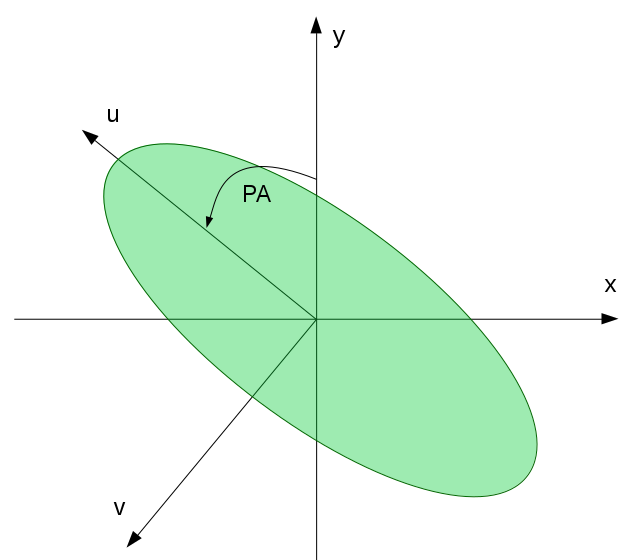
\includegraphics[width=0.5\linewidth]{coord.png}
  \end{center}
  
	Dans le code PROFCL plusieurs systèmes de coordonnées sont utilisés suivant que l'on considère des amas circulaires ou elliptiques. On en fait ici la synthèse.
    \subsection{Coordonnées de référence}
    		Le premier jeu de coordonnées utilisé est celui à partir duquel sont défini les positions des amas et des galaxies dans les simulations académiques et semi-analytiques. Les coordonnées utilisées sont les coordonnées équatoriales $(x, y)$ où $\bm{\hat{x}}$ pointe vers l'Ouest et $\bm{\hat{y}}$ vers le Nord.\par
    		De fait si l'on appelle $RA, Dec$ respectivement l'ascension droite, la déclinaison d'une galaxie alors on a les relations
    		
    		\begin{align*}
    			x & = - (RA - RA_{\rm{cen}})  \cos( Dec ) \\
    			y & = Dec - Dec_{\rm{cen}}
    		\end{align*}
    		
    	\subsection{Coordonnées locales elliptiques centrées}
    		Pour les amas elliptiques centrés il est utile de définir des nouvelles coordonnées $(u, v)$ liées à l'amas définies telles que $\bm{\hat{u}}$ soit aligné le long du demi-grand axe de l'ellipse en direction du Nord à $PA$ nul et $\bm{\hat{v}}$ le long du demi-petit axe en direction de l'Est à $PA$ nul.\par
    		Ainsi les nouvelles coordonnées s'écrivent
    		
    		\begin{align*}
    			u & = - x \sin (PA) + y \cos (PA) \\
    			v & = -x \cos (PA) - y \sin (PA)
    		\end{align*}
    		
    		Le rayon projeté réel est naturellement donné par $R = \sqrt{u^2 + v^2}$. Cependant, lors du traitement des amas elliptiques on est amené à "circulariser" l'amas pour pouvoir en extraire les probabilités de position des galaxies. Cela revient en pratique à "décompresser" l'amas selon son demi-grand axe en le divisant par un facteur $1-e$, i.e. en définissant une nouvelle coordonnée $v^{'} = v/(1-e)$. Il est alors pratique de définir un rayon elliptique comme
    		
    		\begin{equation}
    			\mathscr{R} = \sqrt{u^2 + {v^{'}}^2} = \sqrt{u^2 + \left ( \frac{v}{1-e} \right ) ^2}
    		\end{equation}
    		



\section{Exemple d'amas AMICO}
  \label{Amas}

    \vspace{-10pt}
    \begin{figure}[H]
      \begin{minipage}[t]{0.48\textwidth}
      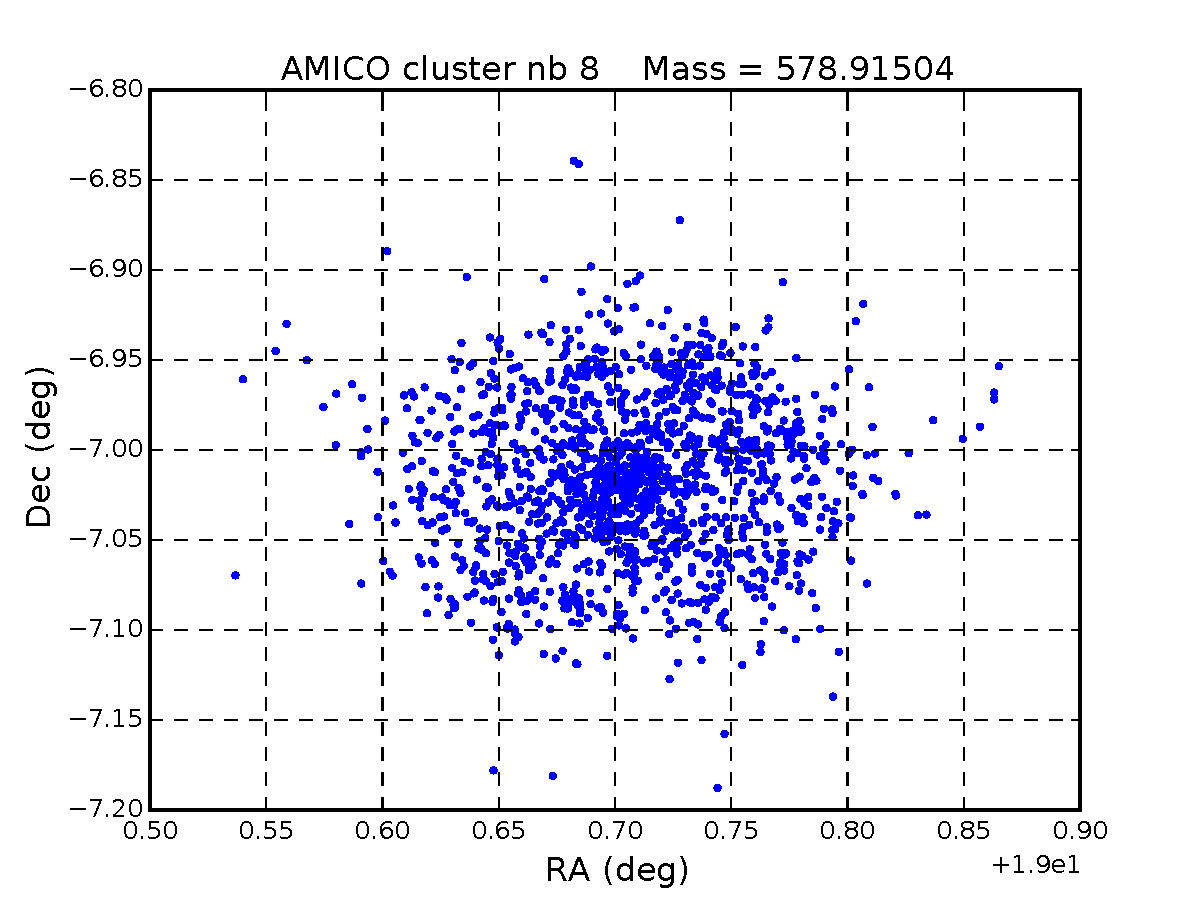
\includegraphics[width=\linewidth]{8.pdf}
  	  \end{minipage}
	  \hfill
    \begin{minipage}[t]{0.48\textwidth}

      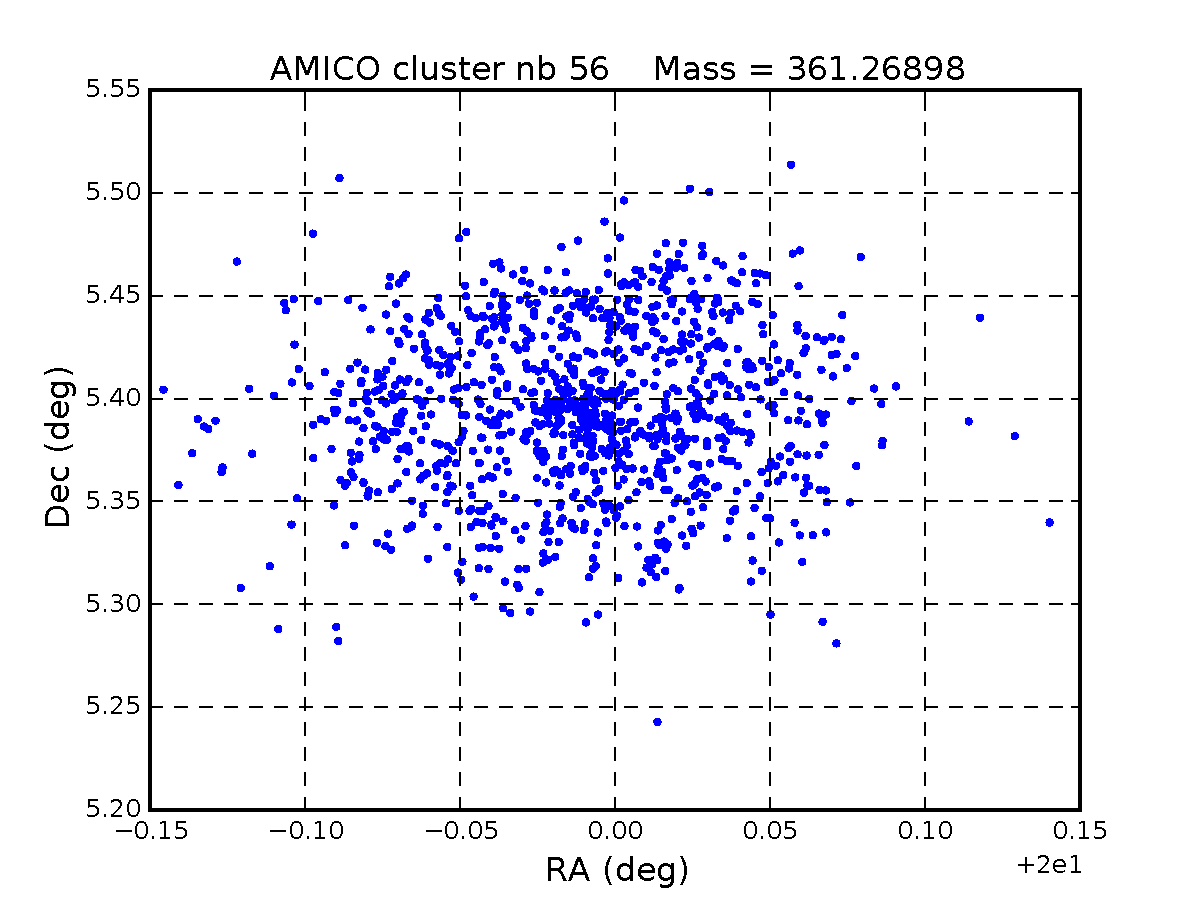
\includegraphics[width=\linewidth]{56.pdf}
  	\end{minipage}
  	
  	\vspace{-5pt}
  	
  	\begin{minipage}[b]{0.48\textwidth}
		  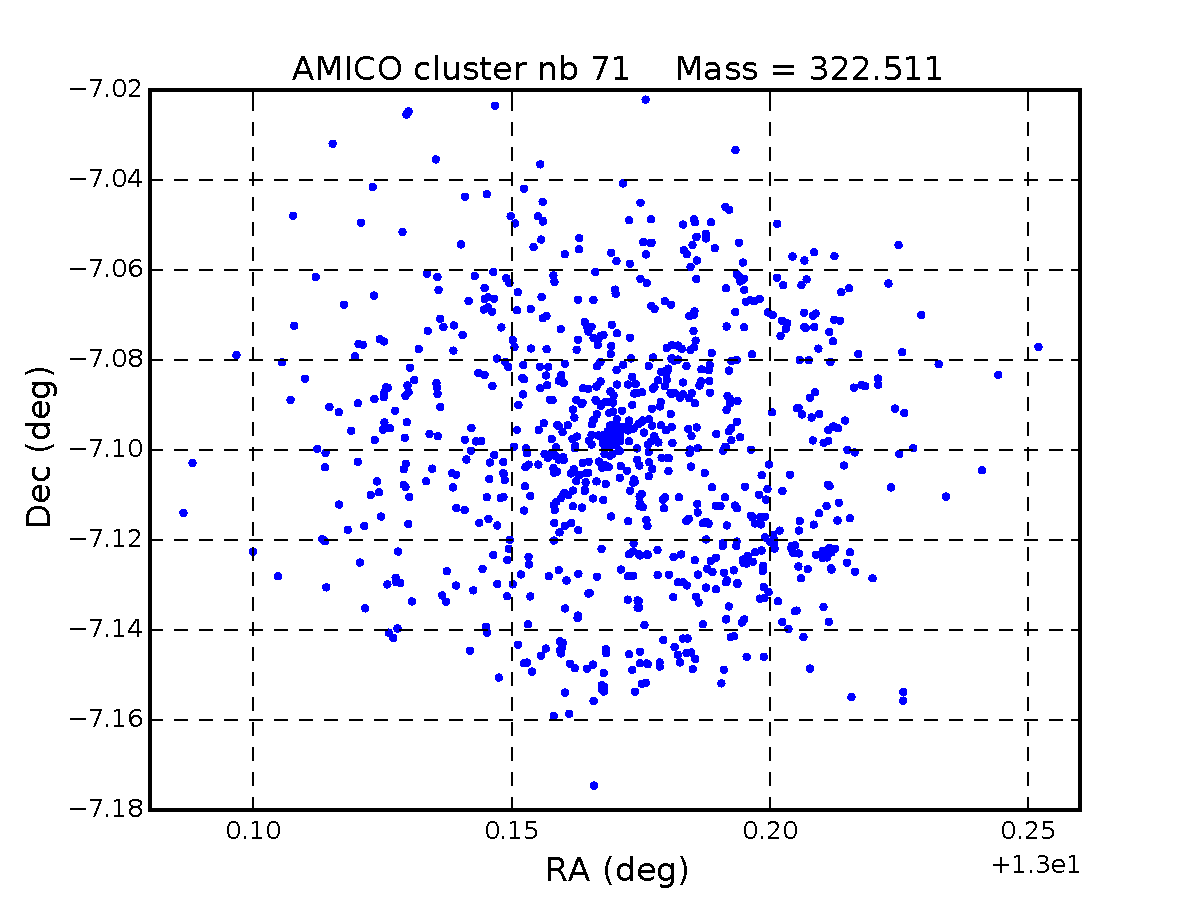
\includegraphics[width=\linewidth]{71.pdf}
    \end{minipage}
		\hfill
		\begin{minipage}[b]{0.48\textwidth}
		  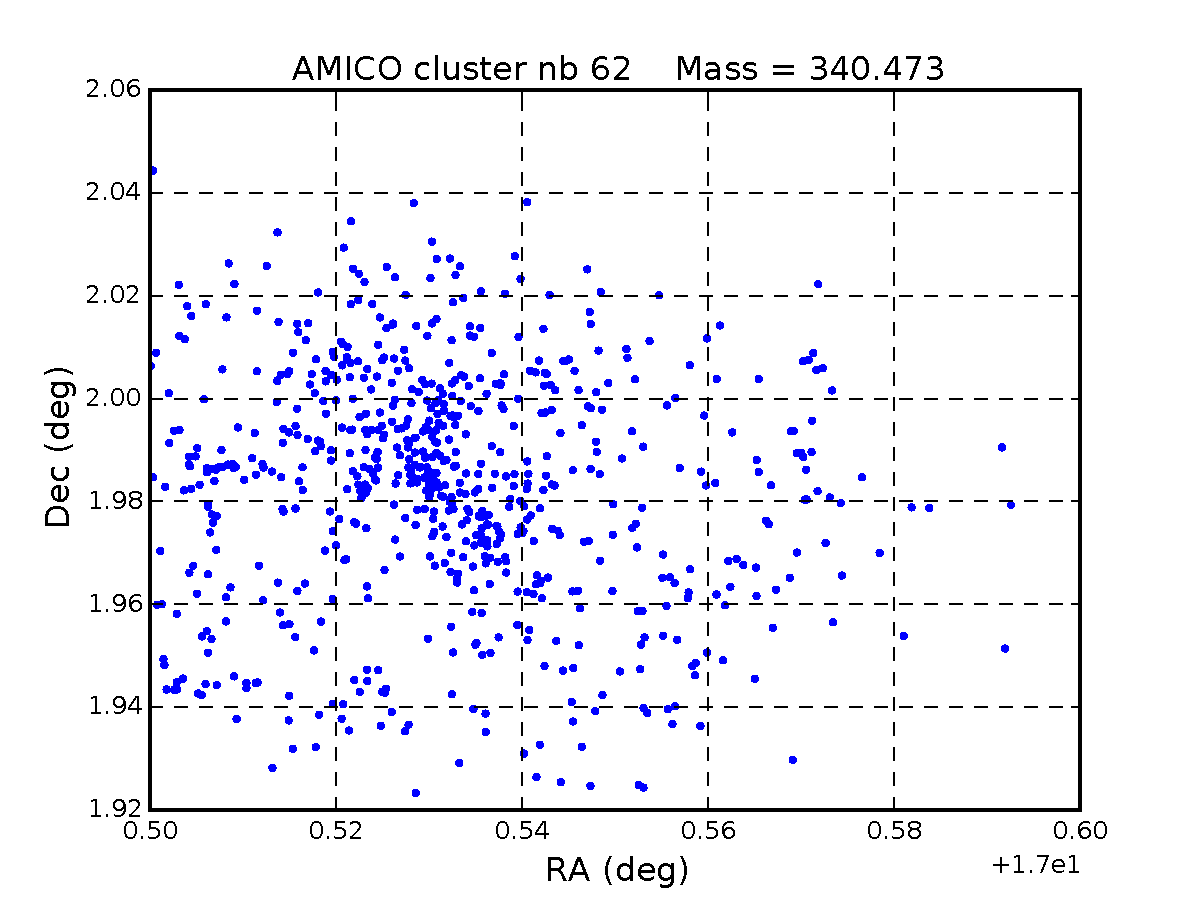
\includegraphics[width=\linewidth]{62.pdf}
  	\end{minipage}
  	
  	\vspace{-5pt}
  	
  	\begin{minipage}[t]{0.48\textwidth}
      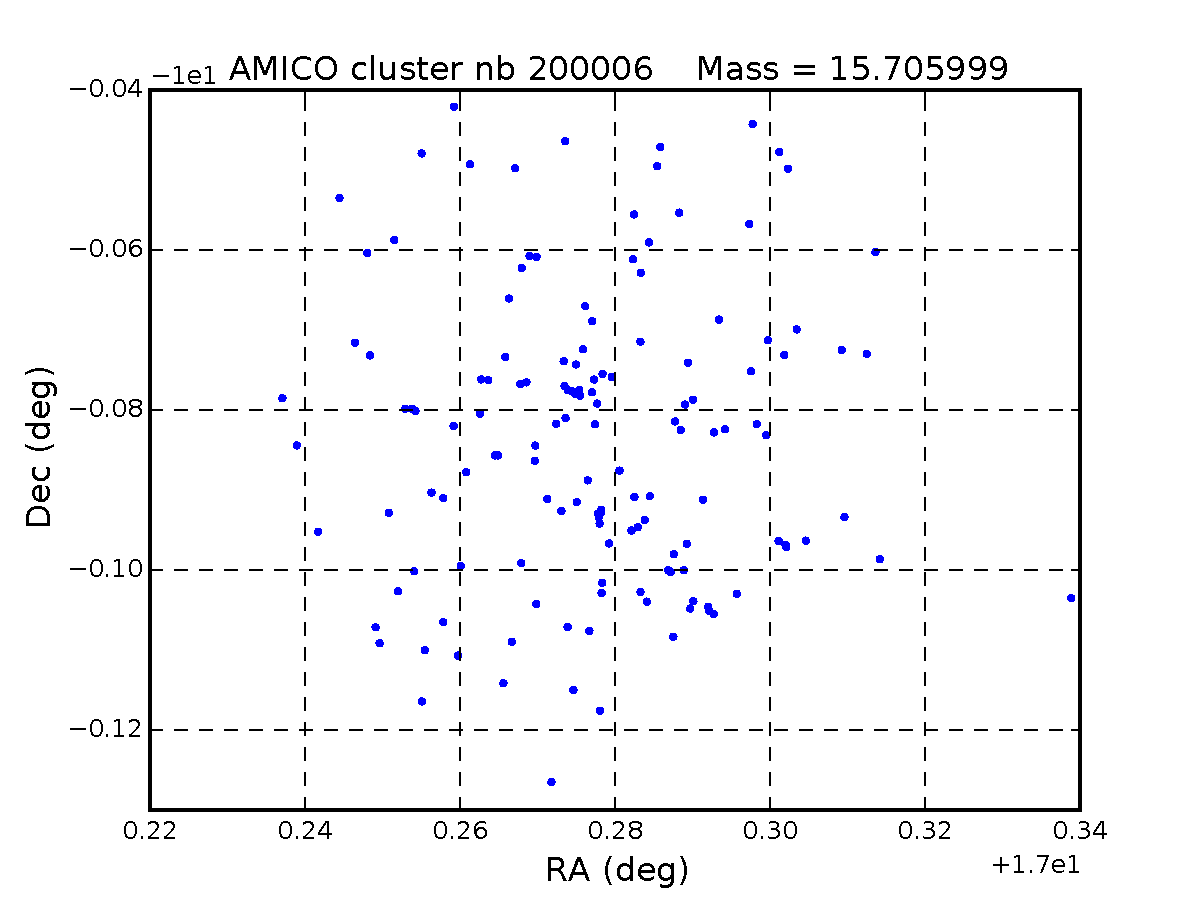
\includegraphics[width=\linewidth]{200006.pdf}
  	  \end{minipage}
	  \hfill
    \begin{minipage}[t]{0.48\textwidth}

      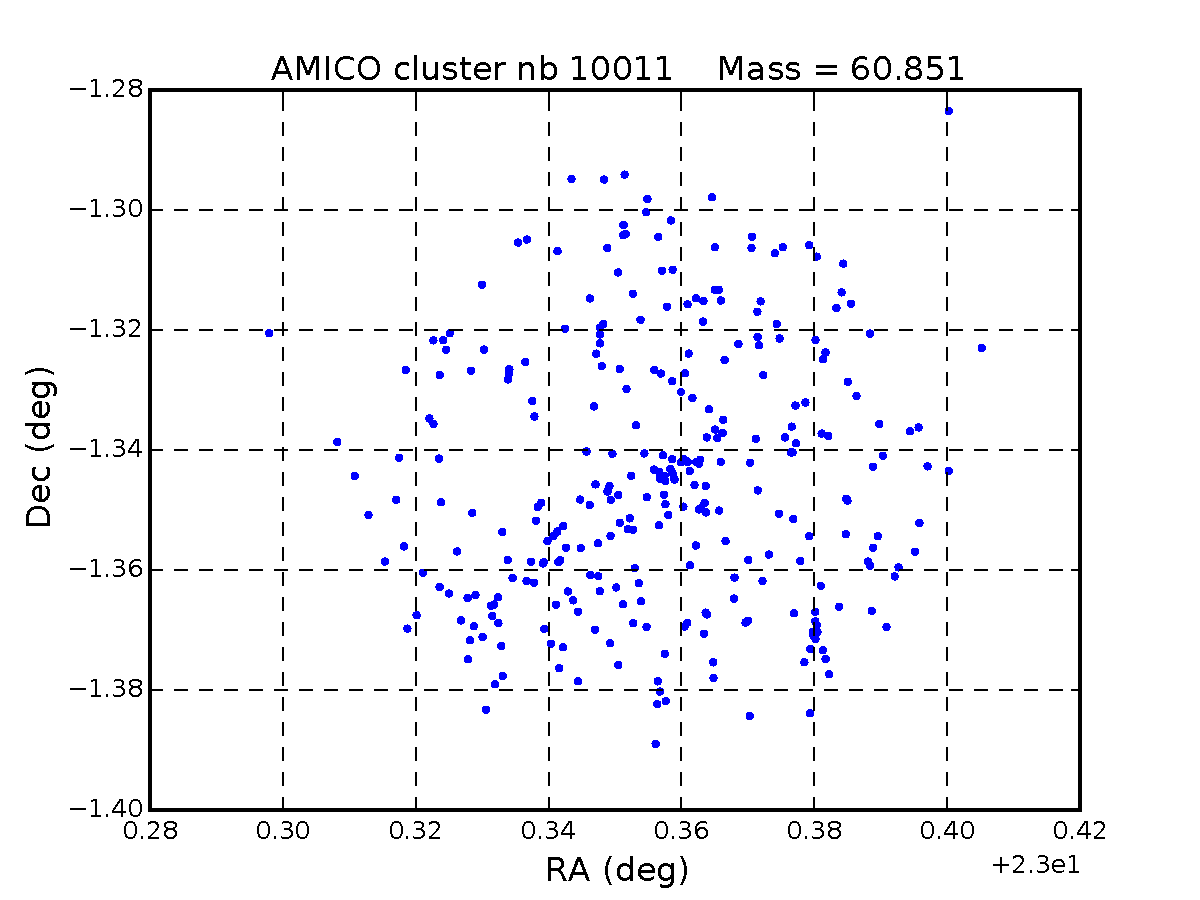
\includegraphics[width=\linewidth]{10011.pdf}
  	\end{minipage}
  	
  	\vspace{-5pt}
  	
  	\begin{minipage}[b]{0.48\textwidth}
		  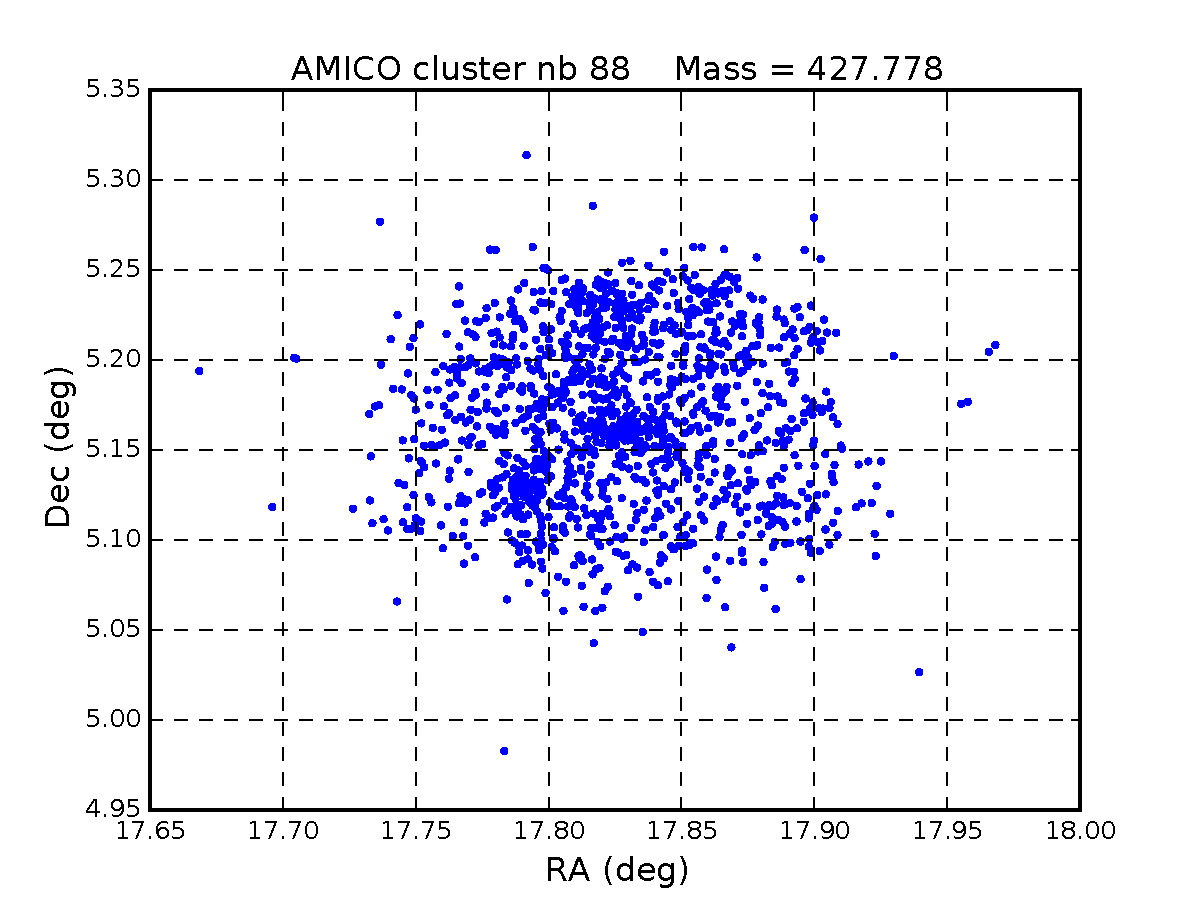
\includegraphics[width=\linewidth]{88.pdf}
    \end{minipage}
		\hfill
		\begin{minipage}[b]{0.48\textwidth}
		  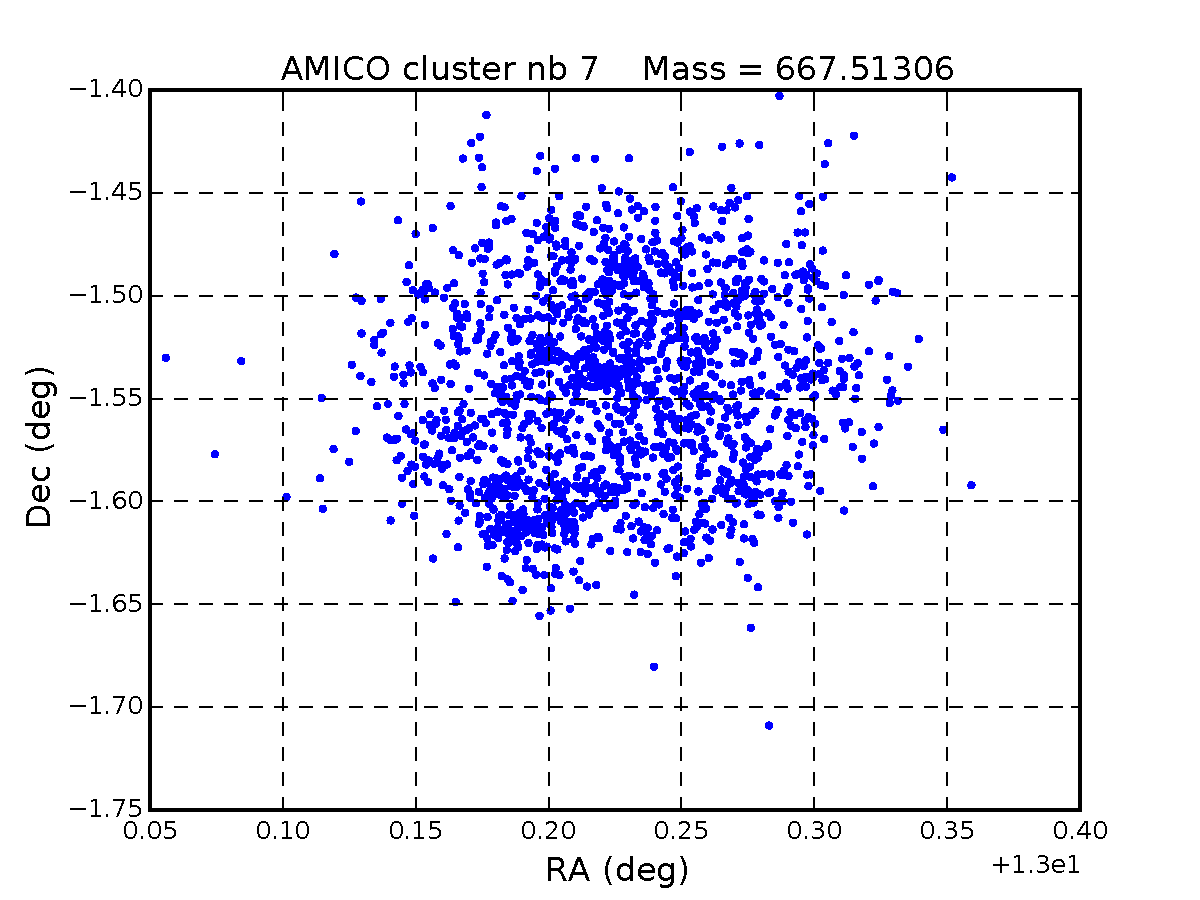
\includegraphics[width=\linewidth]{7.pdf}
  	\end{minipage}
  \end{figure}
    
\end{document}
